
\chapter{Gyrokinetic practice}

\section{Normalisations} 
\label{sec:normalisation}

Of course, all quantities in the code are normalised to typical reference quantities. 
This section will first describe the normalisation for the local (fluxtube) case. Afterwards differences for the global case are pointed out.

The reference quantities chosen for GKW are\\
\begin{tabular}{rl}
  \label{eq:refquantities}
  $\rho_\tref $ : & reference larmorradius \\
  $m_\tref $ : & reference masse \\
  $v_{thref}$ : & reference therm. velocity \\
  $n_\tref $ : & reference number density \\
  $T_\tref $ : & reference temperature \\
  $B_\tref $ : & reference magnetic field \\
  $R_\tref $ : & reference major radius \\
\end{tabular}

These are related with each other by 
\begin{align}
T_{\rm ref} &= \frac{1}{2} m_{\rm ref} v_{\rm thref}^2  
\label{eq:normalise-Tref}
\\
\rho_{\rm ref} &= {m_{\rm ref} v_{\rm thref} \over e B_{\rm ref}} = \frac{2T_\tref}{eB_\tref v_{th\tref}}.
\end{align}
The unit of temperature is energy. Then the symbol $k$ is used for
wavenumbers.  Naturally, the code uses only normalized quantities, and
physical units can only be obtained through the reference quatities.
These quantities are never explicitly specified. The numerical
solution is valid for any choice of these quantities. Note though that
the collision frequency leads to an additional constraint 
\eqref{eq:refquantities-collisions-constraint} between the
quantities mentioned above.
A further constraint exists with finite $\beta = \beta_\tref \beta_N$, where 
\begin{equation} 
\label{eq:betaref}
\beta_{ref} = {n_{\rm ref} T_{\rm ref} \over B_{\rm ref}^2 / 2 \mu_0} .
\end{equation}

There are a couple of normalised dimensionless quantities that are independent of the species. These are the
normalised Larmor radius
\begin{equation} 
\rho_* = \rho_{\rm ref} / R_{\rm ref} \qquad \leadsto  \rho_* = \frac{\rho_\tref }{R_\tref } = \frac{m_\tref v_{thref}}{eB_\tref R_\tref } .
\label{eq:normalise-rho}
\end{equation}
and the fields 
\begin{align} 
\phi = \rho_* {T_{\rm ref} \over e} \phi_N ,
\qquad 
A_\parallel = B_{\rm ref} R_{\rm ref} \rho_*^2 A_{\parallel N} ,
\qquad 
B_{1\parallel} = B_{\rm ref} \rho_* B_{1\parallel N}
\qquad
\chi = \rho_* {T_{\rm ref} \over e} \chi_N ,
\qquad
\Phi = {T_{\rm ref} \over e} \Phi_N ,
\label{eq:phi-norm}
\end{align} 
Here the index $N$ refers to a normalised quantity. 
Note that factors of $\rho_*$ have been added in the definitions of the normalised perturbed fields. 
These factors are chosen such that the normalised quantities are of the order 1. 

Also the parameters time $t$, magnetic field $B$, reference frame angular rotation frequency $\Omega$, and the major radius $R$, are made dimensionless using the reference values 
\begin{align}
&t = { R_{\rm ref} } t_N / v_{\rm thref} , \qquad &B = B_{\rm ref} B_N , \cr 
\noalign{\vskip 0.2 truecm} 
&\Omega = {v_{\rm thref} } \Omega_N / R_{\rm ref},  \qquad &R = R_{\rm ref} R_N .
\label{eq:normalise-parameters}
\end{align}

On the other hand, there are quantities which describe species.
Here, the reference values are used to define, for each species, a dimensionless mass $m_R$, a dimensionless thermal 
velocity $v_R$, a dimensionless density $n_R$, a dimensionless temperature $T_R$, background flow velocity $R\omega$ and a dimensionless centrifugal energy $\cfenn$.
The index $R$ refers to a normalised quantity with species dependence. 
\begin{align} 
m &= m_R m_{\rm ref}
\\
v_{\rm th} &=  v_R v_{\rm thref}
\\
n_{R_0} &= n_R n_{\rm ref} 
\\
T &= T_R T_{\rm ref} \qquad\leadsto T_R = m_Rv_R^2
\label{eq:normalise-T}
\\
\omega &= \frac{v_{\rm thref} }{R_\tref} \omega_N
\end{align}
Since it is not as obvious as the above, we elaborate on the centrifugal potential $\cfen$ with more detail:
\begin{align}
\\
 \cfen &= Ze \Phi - \frac{1}{2}m\Omega^2(R^2 - R_0^2)
\nonumber\\ 
& = Ze\frac{T_\tref }{e}\Phi_N - \frac{1}{2}m_\tref m_R\frac{v_{thref}^2}{R_\tref ^2}\Omega_N^2R_\tref ^2(R_N^2-R_{0N}^2) \nonumber\\
 & =  \left(Z\Phi_N - m_R\Omega_N^2(R_N^2 - R_{0N}^2)\right) T_\tref\nonumber\\
 \cfen &=\cfenn T_{\rm ref}
\label{eq:normalise-cfen}
\end{align} 
The GKW code defines a ``centrifugal energy'' array \texttt{cfen} which contains a temperature factor
\begin{align}
  \mathtt{cfen} = \frac{\mathcal{E}_R}{T_R}
\label{eq:cfen-vs-ER}
\end{align}
such that
\begin{align}
  \mathcal{E}_\Omega = \mathtt{cfen}\cdot T_RT_\tref
\end{align}

The velocity space coordinates are made dimensionless with the help of 
the thermal velocity $v_{th}$ of the respective species 
\begin{align}
  \label{eq:normalisation-velocityspace}
  v_\parallel &= v_{th}v_{\parallel N} = v_{thref} v_R v_{\parallel N} \\
\mu &= \frac{1}{2}\frac{mv_\perp^2}{B}  \nonumber\\
&= \frac{1}{2}\frac{m_\tref m_R(v_{thref}v_R)^2v_{\perp N}^2}{B_\tref B_N} \nonumber\\
&= \frac{m_\tref m_Rv_{thref}^2v_R^2}{B_\tref } \frac{1}{2}\frac{v_{\perp N}^2}{B_N}
= \frac{mv_{th}^2}{B_\tref } \mu_N 
= \frac{2T_\tref T_R}{B_\tref } \mu_N 
\label{eq:normalisation-velocityspace-mu}
\\
J_v &= \frac{2\pi B}{m} = \frac{B_\tref}{m} 2\pi B_N \quad\leadsto  J_{vN} = 2\pi B_N\\
\ud^3 v &= J_v \ud v_{\parallel} \ud\mu = v_{th}^3 \ J_{v,ref}J_{vN}\ \ud v_{\parallel N}\ \frac{m}{B_\tref }\ud\mu_N \quad\text{and with } J_{v,ref}\frac{m}{B_\tref } = 1 \nonumber\\
&= v_{th}^3 J_{vN}\ \ud v_{\parallel N}\ \ud\mu_N = v_{th}^3\ud^3v_N
\end{align}
It is worth to stress that the velocity is normalised by the thermal velocity of each of the species. 
This has the advantage that the grid in velocity space can always be defined relative to the thermal 
velocity. 
Quantities like the potential in \eqref{eq:phi-norm}, however, must be normalised by a reference temperature since it is 
species independent. 
A similar argument applies to the vector potential and the time. 

Note that the magnetic moment $\mu$ is normalised such that the
particle mass $m_R$ (which differs greatly between electrons and ions)
is not part of $\mu_N$. This makes the grid used in the code be
actually a $mu_N/m$ grid, which has the same values for all
species. When a quantity is integrated over velocity space, this does
not alter the result.
FIXME The code not even uses \texttt{bn} for $B_N$, but puts a 1?|

It is then convenient to normalise the distribution functions according to 
\begin{equation} 
f = \rho_* {n_{R_0} \over v_{\rm th}^3} f_N ,
\qquad 
F_M = {n_{R_0} \over v_{\rm th}^3} F_{MN} .
\end{equation} 
The gradient of density and temperature are made dimensionless using the density and 
temperature of the species under consideration, but the plasma rotation 
is largely a bulk motion of all the species together and its gradient is normalised using  
the reference thermal velocity $v_{\rm thref}$
\begin{equation} 
\label{eq:gradients}
{1 \over L_{n,N}} = {R_{\rm ref} \over L_n} = - {1\over n_{R_0}} \pd{ n_{R_0} }{\psi} ,
\qquad 
{1 \over L_{T,N}} = {R_{\rm ref} \over L_T} = - {1 \over T} \pd{ T }{\psi} , 
\qquad 
u^\prime_N = - {R_{\rm ref} \over v_{\rm thref}} \pd{ \omega_\phi}{\psi} .
\end{equation}
The gradient length scales are normalised with $R_{\rm ref}$, but note that the same quantities are often written 
as $R/L_n$ and $R/L_T$ elsewhere in the literature.  Note also that the radial coordinate $\psi$ is normalised:
\begin{equation}
 \label{eq:psi-def}
 \psi = \frac{R_{\rm max}-R_{\rm min}}{2R_{\rm ref}},
\end{equation}
where $R_{\rm max}$ ($R_{\rm min}$) is the maximum (minimum) major radius of the flux 
surface. 
For circular surfaces, for instance, $\psi = r / R_{\rm ref} = \epsilon$, 
where $r$ is the minor radius.  For the $s-\alpha$ geometry, you can take $R_{\rm ref}$ to have any 
value you like, but it is simplest to always use the magnetic axis. For the Circ, Miller and Chease $R_{\rm ref}$ 
has a specific meaning defined by the geometry.
All gradients are normalised using the major radius $R_{\rm ref}$,
i.e.
\begin{equation} 
\nabla = {1\over R_{\rm ref}} \nabla_{N} .\qquad 
\end{equation} 
The poloidal flux $\Psi$ used in the derivation of the metric tensors is normalised according to
\begin{equation} 
 \Psi = R_{\rm ref}^2 B_{\rm ref}\Psi_N .
\end{equation}

The strength of the electromagnetic effects is determined by the plasma beta $\beta$.  
Although $\beta$ is dimensionless we define a different dimensionless beta $\beta_{ref}$ for the 
use in the code. This $\beta_{ref}$ is directly related to the reference values via \eqref{eq:betaref}.


Finally, the wave vectors introduced in the spectral representation arise from the perpendicular
gradient of a fluctuating quantity and will therefore be normalised to $\rho_{\rm ref}$:
\begin{align} 
k_\psi = \frac{k_{\psi N}}{\rho_{\rm ref}} \qquad 
k_\zeta = \frac{k_{\zeta N}}{\rho_*} \qquad 
\label{eq:kN}
\end{align}
In the later sections we will, of course, use only the normalised quantities. 
The index $N$ is then dropped for convenience. 

\subsection{Normalisation for the Global Case}
\label{sec:normalisation-global-specialities}

\subsubsection*{Grid Temperature and Grid Density}
\label{sec:grid-temp-grid-dens}

In the local version of GKW the velocity coordinates are normalized to the thermal velocity 
of the considered species background. \index{Normalization} 
This has the advantage that the Maxwellian can be represented with the same accuracy for 
each of the species even if the temperatures of the species are very different. 
When the background temperature is a function of the radial coordinate, however, the thermal velocity is no 
longer a constant. 
Using the local thermal velocity for normalization would have the advantage that the Maxwell 
is represented with the same relative resolution at each radial point, but would make the 
normalization constant a function of radius, and would lead to cross terms in all radial 
derivatives. A choice has therefore been made to use a fixed temperature, often the temperature at 
one particular radial location, for the normalization. This has the advantage that it does not change the structure 
of the equations, but also has disadvantages. In the global case the grid must be, both set up 
such that it is big enough to represent the maximum temperature ($T_{\rm max}$) in the domain, as well as 
have sufficient resolution to resolve the distribution function of the smallest temprature
($T_{\rm min}$). Because the velocity scales as the square root of the temperature this increases 
the computational cost by a factor $T_{\rm max} / T_{\rm min}$ over a local simulation. 


The temperature used for the normalization of the velocity coordinates
is the 'grid temperature' $T_G$, instead of $T_\tref$ directly. 
$T_G$ is not dimensionless but has physical units, just like $T_\tref$. $T_G$ is
not a function of the radius but, unlike $T_{\rm ref}$, is different
for each species.  The corresponding thermal velocity used for normalization is then $w$.
\begin{equation}
T_G = \frac{1}{2} m w^2 \qquad w = \sqrt{\frac{2 T_G}{m} }
\end{equation}
Where $m$ is the particle mass of the respective species. 
That is, while in the local case the velocity is normalised to the same $v_{th\tref}$ (related to a $T_\tref$)
for all species, for the global case $v_{th\tref}$ is replaced by a reference velocity $w$ (related to 
a new temperature, the species grid temperature $T_G$).

Species background temperature $T$ and species grid temperature $T_G$ are normalized with $T_{\rm ref}$
\begin{equation}
T_G = T_{GR} T_\tref \qquad T = T_R T_\tref
\end{equation}
and since $T_{\rm ref}$ is connected to the reference thermal velocity $v_{th\tref}$ via \eqref{eq:normalise-Tref} we have 
\begin{align}
w &= w_R v_{thref} \\
w_R &= \frac{w}{v_{thref}} 
=\frac{1}{v_{thref}} \sqrt{\frac{2T_G}{m}}
\nonumber\\
&=\frac{1}{v_{thref}} \sqrt{\frac{2T_{GR}T_\tref}{m}}
\\
&=\sqrt{\frac{ m_\tref}{2T_\tref} } \sqrt{\frac{2T_{GR}T_\tref}{ m_Rm_\tref} } 
= \sqrt{\frac{T_{GR}}{ m_R} } \qquad \leadsto T_{GR} = m_Rw_R^2
\end{align}
By normalising the species thermal velocity to $w$ we have
\begin{align}
  v_{th} &= v_R w\\
&= v_Rw_Rv_{th\tref} 
= \sqrt{\frac{T_R}{m_R}}\sqrt{\frac{T_{GR}}{m_R}}v_{th\tref}
= \frac{\sqrt{T_RT_{GR}}}{m_R}v_{th\tref}
\end{align}
The velocity space coordinates for the respective species are
\begin{align}
v_\parallel = v_{\parallel N} v_R w  \qquad \mu = \frac{ mw^2}{B_{\rm ref}} \mu_N 
\end{align}

To see some relations this implies, consider the normalisation of the
species temperature $T$:
\begin{align}
  T &= \frac{1}{2}m v_{th}^2 \\
&= \frac{1}{2}m_Rm_\tref v_R^2w_R^2v_{th\tref}^2  
 = v_R^2 m_Rw_R^2 \frac{1}{2}m_\tref v_{th\tref}^2  
\\
 &= \frac{T_R}{m_R} T_{GR} T_\tref
\end{align}
Another relationship is
\begin{align}
  \frac{T_R}{T_{GR}} &= \frac{T_RT_\tref}{T_{GR}T_\tref} = \frac{T}{T_G}
\\
&= \frac{\frac{1}{2}mv_{th}^2}{\frac{1}{2}mw_{th}^2}
= \frac{v_R^2w_R^2v_{th\tref}^2}{w_R^2v_{th\tref}^2}
= v_R^2
\label{eq:normalise-vR-Tratio}
\end{align}


Note that only the velocity space coordinates are normalized with the grid thermal velocity $w$. 
Species independent quantities and parameters, like time, rotation velocity and normalized Larmor radius 
continue to be normalized using 
$v_{\rm thref}$ , in the global case, according to \eqref{eq:normalise-rho} and \eqref{eq:normalise-parameters}.
Accordingly, the fields are also normalized with $T_{\rm ref}$ like in \eqref{eq:phi-norm}.

Besides the temperature, a similar normalization is used for the density. Each of the species 
is normalized to the 'grid density' $n_G$ which is not a function of the radius but, unlike $n_\tref$ is different for each species. 
\begin{equation}
n_G = n_{\rm ref}n_{GR}  \qquad n_{R_0} = n_{R}n_{\rm ref}
\end{equation}

The the potential $\cfen$ contains the frame rotation frequency $\Omega$ which we would like to keep a konstant by all means (cf. section \ref{sec:global-plasma-rotation}). Likewise, $\omega$ continues to be normalised like in \eqref{eq:normalise-parameters}.
\begin{align}
\omega &= \frac{v_{th\tref}}{R_\tref} \omega_N 
= \frac{w}{w} \frac{v_{th\tref}}{R_\tref} \omega_N 
= \frac{w}{w_Rv_{th\tref}} \frac{v_{th\tref}}{R_\tref} \omega_N 
= w \frac{1}{w_R} \frac{1}{R_\tref} \omega_N 
= \frac{w}{R_\tref}  \sqrt\frac{m_R}{T_{GR}} \omega_N 
\end{align}

\emph{Please note, the implementation of plasma rotation $\Omega$ in
  the global case is not entirely consistent and using the plasma
  rotation $\Omega$ in the global case is strongly discouraged. Please
  see also the comments on this in
  section~\ref{sec:global-normalisation}.}

% \begin{equation}
%  {\cal E}_\Omega = {\cal E}_{\Omega N} T_{R} 
% \label{eq:normalise-cfen-global}
% \end{equation}
% FIXME This text used to list $\Omega = v_{\rm thref} \Omega_N / R_\tref$ and ${\cal E}_\Omega = {\cal E}_{\Omega N} T_{G}$,i.e. the frame rotation is species 
% independent, just like for fluxtube. If we then normalise $\cfen$ with $T_G$, this introduces a 
% species-dependence in the normalisation of $\Omega$ inside $\cfen$ while there is none for $\Omega$ 
% elsewhere, which looks inconsistent to SRG. However, this seems to be used in the Maxwellian below.|

% FIXME $\beta_\tref$ depends on $T_\tref n_\tref$. Is this replaced by a kind of 'grid beta' or not, and does one need an argument for it?|

It is to be noted that the 'old' flux-tube normalization is included in the global normalization above if one sets $T_G \equiv T_\tref$ and $n_G \equiv n_\tref$.

\paragraph{Example: Normalisation of the Maxwellian Background Distribution} 
\label{sec:global-normalisation}
In the global case, there are a couple of difficulties concerning the normalisation, so that the normalisation scheme is not totally identical to that of the local (fluxtube) case.
This is described in detail in section~\ref{sec:normalisation-global-specialities}.

For the global case, with its adapted normalization, the Maxwellian from \eqref{eq:maxwell} 

\begin{align} 
F_{M} &= {n_{R_0} \over \pi^{3/2} v_{\rm th}^3 } \exp 
\biggl [ - {(v_\parallel-(R B_t/B)\omega_\phi )^2 + 2 \mu B / m \over v_{\rm th}^2} - \cfen/T \biggr ]
\end{align}
becomes \index{Maxwell distribution} 
\begin{align}
  F_{M,\mathrm{global}} 
 &=\frac{n_Rn_\tref }{ \pi^{3/2} (v_Rw)^{3} } \exp \left [ - \frac{ 
\left(v_{\parallel N}v_Rw - R_\tref R_N B_{tN} \frac{w}{R_\tref}\sqrt\frac{m_R}{T_{GR}}\omega_{\phi N} / B_N\right)^2 + 2 \frac{mw^2}{B_\tref}\mu_N B_\tref B_N\frac{1}{m} 
}{ (v_R w)^2}
- 
\frac{T_\tref\mathcal{E}_R}{T_\tref T_R}  \right ] 
\nonumber\\
 &=\frac{n_\tref}{w^3} \frac{n_R }{ \pi^{3/2} v_R^3 } \exp \left [ - \frac{ 
\left(v_{\parallel N}v_R - \sqrt\frac{m_R}{T_{GR}}R_N B_{tN} \omega_{\phi N} / B_N\right)^2 + 2 \mu_N B_N
}{ v_R ^2}
- 
\frac{\mathcal{E}_R}{T_R}  \right ] 
\\
F_{M,\mathrm{global}}&=\frac{n_\tref}{w^3} \frac{n_R }{ \pi^{3/2} v_R^3 } \exp \left [ - \frac{ 
\left(v_{\parallel N}v_R - \sqrt\frac{m_R}{T_{GR}}R_N B_{tN} \omega_{\phi N} / B_N\right)^2 + 2 \mu_N B_N
}{ v_R ^2}
- 
\frac{\mathcal{E}_R}{T_R}  \right ] 
\end{align}
We replace $v_R$ with \eqref{eq:normalise-vR-Tratio}.
\begin{align}
  F_{M,\mathrm{global}}&=\frac{n_G}{w^3}\frac{n_R }{n_{GR} \pi^{3/2} (T_R/T_{GR})^{3/2} } \exp \left [ - \frac{ 
\left(v_{\parallel N}v_R - \sqrt\frac{m_R}{T_{GR}}R_N B_{tN} \omega_{\phi N} / B_N\right)^2 + 2 \mu_N B_N
}{ T_R/T_{GR}}
- 
\frac{\mathcal{E}_R}{T_R}  \right ] 
\label{eq:maxwellian-global}
\end{align}
In order to draw a grid density $n_G$ out of the distribution, we have expanded the prefactor with $n_{GR}$ here.
In the Maxwellian \eqref{eq:maxwellian-global} above, the quantities
$n_R$, $T_R$, $R_N$, $\omega_{\phi N}$, $\mathcal{E}_R$ and
$B_{tN},B_N$ are functions of radius.

In this sense, the distribution functions are normalized as follows 
\begin{align} 
F_M &= 
\frac{n_G}{ w^3} F_{MN} \\
f &= \rho_* \frac{n_G}{w^3} f_N
\end{align}

Due to the implementation of \texttt{cfen} from \eqref{eq:cfen-vs-ER}, the code has
\begin{align}
  F_{M,\mathrm{global}}&=\frac{n_G}{w^3}\frac{n_R }{n_{GR} \pi^{3/2} (T_R/T_{GR})^{3/2} } \exp \left [ - \frac{ 
\left(v_{\parallel N}v_R - \sqrt\frac{m_R}{T_{GR}}R_N B_{tN} \omega_{\phi N} / B_N\right)^2 + 2 \mu_N B_N
}{ T_R/T_{GR}}
- 
\mathtt{cfen} \right ] 
\end{align}

(This is the previous version of the global normalisation of the
Maxwellian given here, but SRG thinks there is something wrong with it:
\begin{align}
F_{MN,orig}&= \frac{n_{GN}}{1} \frac{n_N }{ \pi^{3/2} (T_N / T_{GN})^{3/2} } \exp \left [ - \frac{ 
(v_{\parallel N} - \sqrt{m_N/T_{GN}} R_N B_{tN} \omega_{\phi N} / B_N)^2 + 2 \mu_N B_N + 
{\cal E}_{\Omega N} }{ T_N / T_{GN}} \right ] 
\end{align}
)

Just like \eqref{eq:maxwell}, the Maxwellian here in
\eqref{eq:maxwellian-global} integrates to the background density and
background temperature. The exp. factor modifies the momenta because
the distribution has a dependence on the poloidal angle $\theta$ if the frame rotates.
\begin{align}
\int F_M \, {\rm d}^3 {\bf v} &= n_{R_0} \exp\left(-\frac{\mathcal{E}_\Omega (\theta)}{T}\right) & \int F_{MN} \, {\rm d}^3 {\bf v} &= \frac{n_{R}}{n_{GR}} \exp\left(-\frac{\mathcal{E}_\Omega}{T}\right)
\\
\int \frac{1}{ 2} m v^2 F_M \, {\rm d}^3 {\bf v} &= \frac{3 }{ 2} T \exp\left(-\frac{\mathcal{E}_R(\theta)}{T_R}\right)
&
\int \frac{1}{ 2} m v^2 F_{MN} \, {\rm d}^3 {\bf v} &= \frac{3 }{ 2} T_R \exp\left(-\frac{\mathcal{E}_R}{T_R}\right)
\end{align}


\section{Geometry}
\label{geometry}
GKW is formulated in field aligned Hamada coordinates \cite{HAM62}, i.e. the contravariant
components of both the poloidal $B^s$ and toroidal magnetic field $B^\gamma$
are flux functions. The safety factor is then determined by the ratio $q = B^\gamma / B^s$.  
Starting from an orthogonal coordinate system $(\psi,\theta,\varphi)$, where $\psi$ is the radial
coordinate (i.e. ${\bf B}\cdot \nabla \psi = 0$), $\theta$ is the poloidal angle (upward 
on the outboard midplane), and $\varphi$ is the toroidal angle (clockwise when viewed from 
above), and using the transformations 
\begin{equation} 
s = s(\psi,\theta), \qquad \gamma = \gamma(\psi,\theta,\varphi),
\label{transformations}
\end{equation} 
one can derive \cite{SCO98,SCO01} (see Appendix~\ref{sec:hamada} for more details):
\begin{equation} 
s(\theta,\psi) = {\int_0^\theta {{\rm d} \theta^\prime \over {\bf B} \cdot \nabla \theta^\prime} 
\biggl /  \oint {{\rm d}\theta^\prime \over {\bf B}\cdot \nabla \theta^\prime}} ,
\end{equation}
\begin{equation} 
\gamma = {\varphi \over 2\pi} + s_{\rm B}{R B_t \over 2\pi} \int_0^\theta {{\rm d} \theta^\prime \over {\bf B}
\cdot \nabla \theta^\prime} \biggl [ \biggl \{ {1\over R^2} \biggr \} - {1\over R^2} 
\biggr ] ,
\end{equation} 
with 
\begin{equation} 
B^s =  {1 \biggl /  \oint {{\rm d}\theta^\prime \over {\bf B}\cdot \nabla \theta^\prime}} \qquad 
B^\gamma = s_{\rm B}{R B_t\over 2 \pi } \biggl \{ {1\over R^2} \biggr \}. 
\end{equation}  
In the equations above, the magnetic field is decomposed as
\begin{equation}
{\bf B} = s_{\rm B}RB_t\nabla \varphi + s_{\rm j}\nabla\varphi\times\nabla\Psi ,
\end{equation}
where $B_t>0$ is the toroidal component of the magnetic field, $s_{\rm B}=\pm 1$ and $s_{\rm j}=\pm 1$ the sign of 
the magnetic field and plasma current (positive in the direction of $\nabla \varphi$) and $\Psi$ the normalised poloidal 
flux ($\nabla \Psi$ points from the magnetic axis to the plasma edge).
The brackets $\{ \}$ denote the flux surface average, which in the transformed coordinates 
can be written (more details in \ref{sec.fsa}) as 
\begin{equation} 
\{ g \} = \oint g \,{\rm d}s. 
\end{equation} 
The normalising constants have been chosen such that the domain [-1/2,1/2] in $s$ corresponds 
to one poloidal turn and the domain [-1/2,1/2] in $\gamma$ corresponds to one toroidal turn.
Note that the transformations of Eq.~(\ref{transformations}) leave the angle $\gamma$ to be 
an ignorable coordinate, since any quantity that is independent of $\varphi$ will also be 
independent of $\gamma$ after the transformation.

The coordinates given above are transformed using a simple linear transformation 
\begin{equation} 
\zeta =  q s - \gamma \qquad {\rm where} \qquad q = {B^\gamma \over B^s} 
\end{equation}
to make them field aligned, i.e. ${\bf B} \cdot \nabla = B^s \pd{}{s}$ as $B^\zeta = 0$ and $B^\psi = 0$. 
Note that the coordinate transformation above flips the sign of the toroidal angle. 
The right handed coordinate system can therefore be defined as $(\psi,\zeta,s)$. 
The Jacobian of the new coordinate system can be expressed in terms of the original 
Jacobian through 
\begin{equation} 
J_{\psi  \zeta s} = 2\pi {\bf B} \cdot \nabla \theta \oint {{\rm d} \theta^\prime \over 
{{\bf B} \cdot \nabla \theta^\prime}} J_{\psi \theta \varphi} .
\end{equation} 
We note here that the coordinates $\psi$, $s$ and $\zeta$ are chosen dimensionless with $\psi$ being a normalised 'minor radius' of the flux surface, see Eq.~(\ref{eq:psi-def}).
We shall refer to $\zeta$ as the `bi-normal' coordinate since it is neither strictly toroidal or poloidal.

Close inspection of the gyrokinetic equation~(\ref{Vlasov}) shows that it contains parallel derivatives 
\begin{equation} 
{\bf b} \cdot \nabla  = {{\cal F}} \pd{}{s} \quad \rightarrow \quad 
{\cal F} = {B^s \over B} ,
\end{equation}
and perpendicular drifts, with the latter all involving a cross product with the magnetic field. 
It is then convenient to define the tensor 
\begin{equation} 
\label{efun}
{\cal E}^{\alpha \beta} = {1 \over 2 B} (\nabla x_\alpha \times \nabla x_\beta) \cdot {\bf b}.
\end{equation} 


The convection connected with the velocity ${\bf v}_\chi$ can be directly expressed in 
this tensor times the derivatives of the potential towards $x_\alpha$ and the distribution towards
$x_\beta$.
\begin{align}
  v_\chi\cdot \nabla f &= \frac{(-\nabla\phi)\times \mathbf{b}}{\mathbf{B}} \cdot \nabla f\\
&= \frac{\mathbf{b}\times \frac{1}{\rho_*R_{ref}} 
\nabla_N\rho_*\frac{T_{ref}}{e}\phi_N}{B_{ref} B_N} 
\cdot \frac{1}{\rho_*R_{ref}}\nabla_N \rho_* \frac{n_{R0}}{v_{th}^3}f_N\\
&= \frac{\frac{1}{2}m_{ref}v_{th,ref}^2}{eR_{ref}B_{ref}}
\frac{\mathbf{b}\times\nabla_N\phi_N}{B_N}
\cdot \frac{1}{R_{ref}}\nabla_N \frac{n_{R0}}{v_{th}^3}f_N\\
&= \frac{\rho_{ref}}{R_{ref}}v_{th,ref}
\frac{1}{2}\frac{\mathbf{b}\times\nabla_N\phi_N}{B_N}
\cdot \frac{1}{R_{ref}}\nabla_N \frac{n_{R0}}{v_{th}^3}f_N
\qquad
\text{use } \nabla_N = \mathbf{e}^\alpha \partial_\alpha = \nabla_N x^\alpha\pd{}{ x^\alpha}
\\
&= \rho_*\frac{v_{th,ref}}{R_{ref}}\frac{n_{R0}}{v_{th}^3}
\frac{1}{2}\frac{\mathbf{b}\times\nabla_N x^\alpha \pd{}{ x^\alpha} \phi_N}{B_N}
\cdot \nabla_N x^\beta\pd{}{ x^\beta} f_N\\
&= \rho_*\frac{1}{t_{ref}}\frac{n_{R0}}{v_{th}^3}
\frac{1}{2}\frac{\nabla_N x^\alpha\times\nabla_N x^\beta}{B_N}
\cdot \mathbf{b}  \pd{\phi_N}{x^\alpha} \pd{f_N}{x^\beta} \\
&= \rho_*\frac{1}{t_{ref}}\frac{n_{R0}}{v_{th}^3}
\mathcal{E}^{\alpha\beta}
\pd{\phi_N}{x^\alpha} \pd{f_N}{x^\beta}
\end{align}

It is worth noting that the magnetic field can be expressed as 
\begin{equation}
\label{eq:efun-cst}
 \mathbf{B} = 2\pi s_{\rm j} \nabla \Psi \times \nabla \zeta,
\end{equation}
which immediately leads to 
\begin{equation} 
{\cal E}^{\psi \zeta} = \frac{s_{\rm j}}{4\pi}\pd{\psi}{\Psi},
\label{eq:efun-flux}
\end{equation} 
showing that ${\cal E}^{\psi \zeta}$ is constant on a flux surface. For convenience we define two more quantities 
\begin{equation} 
{\cal D}^\alpha = - 2 {\cal E}^{\alpha \beta} {1 \over B} \pd{ B}{x_\beta}, \qquad 
{\cal G} = {\cal F} \pd{ \ln B}{s} ,
\end{equation}
with ${\cal D}$ related to the grad B drift, and ${\cal G}$ to the trapping. Finally, the Coriolis drift and centrifugal drift will enter the 
equations through the one forms ${\cal H}$ and ${\cal I}$ respectively
\begin{equation} 
{\cal H}^\alpha = -\frac{s_{\rm B}}{B\Omega}{\bf \Omega}_\perp \cdot \nabla x_\alpha, 
\qquad 
{\cal I}^\alpha =  {s_{\rm B} \over 2 B} (\nabla x_\alpha \times \nabla R^2) \cdot {\bf b}
\end{equation}
and the centrifugal potential is calculated (see Sec. \ref{cfphi}) using the quantities
\begin{equation} 
{\cal J} = R^2 - R_0^2, 
\qquad 
{\cal K} = \pd{ {\cal J}}{\psi}\biggr|_s,
%=R\pd{ R}{\psi} + R_0\pd{ R_0}{\psi}
\qquad
{\cal L} = \pd{ (R_0^2)}{\psi}\biggr|_s.
\end{equation}
For transformations of the shearing rate we also define 
\begin{equation}
{\cal M} = \pdd{\Psi}{\psi} = {s_{\rm j} \over 4 \pi}\pd{}{\psi}\left({1 \over {\cal E}^{{\psi \zeta}}}\right).
\end{equation}
The tensor elements defined above all have similar magnitude. It must be realised though that these elements
are multiplied with the derivatives towards the respective coordinate. Since the derivatives along the field 
are much smaller than the derivatives in the perpendicular plane, the tensor elements containing the coordinate
$s$ are usually neglected (i.e. ${\cal D}^s = {\cal E}^{s \psi} = {\cal E}^{s \zeta} = {\cal H}^s = 0$), 
except in the case of those multiplied with the background potential $\Phi$, or when higher $\rho^*$ effects are included.

GKW uses the local limit. Central to this approximation is the small scales of the turbulent fluctuations. 
All background plasma parameters are assumed homogeneous across the simulation domain perpendicular to 
the field, i.e. there is no dependence of the parameters on the coordinates $\zeta$ and $\psi$.  The turbulence is homogeneous 
in the plane perpendicular to the magnetic field and periodic boundary conditions apply.  
Note that the dependence of equilibrium quantities on the 'parallel' coordinate $s$ are kept. 
All the tensors ${\cal D, E, F, G, H, I, J, K, M}$ as well as the metric tensor, are therefore, functions of the
parallel coordinate $s$ only.

\subsection{\texorpdfstring{s-$\alpha$}{s-alpha}}
The simplified `$s-\alpha$' equilibrium (with $\alpha=0$) is directly implemented in the code through pre-defined tensor elements. 
The latter model equilibrium is the simplest choice of the geometry of a tokamak with the flux surfaces being 
circular and having a small inverse aspect ratio $\epsilon = r / R \ll 1$, with $r$ being the 
minor radius of the surface and $R=R_{\rm ref}$.  
Only the lowest order in an $\epsilon$ expansion is kept in the definition of all the tensors. 
The coordinates can then be approximated as 
\begin{equation} 
\psi = \epsilon = {r \over R}, \qquad 
\zeta =  {s_{\rm B} s_{\rm j} \over 2 \pi} [|q| \theta - \varphi ], \qquad 
s = {\theta \over 2 \pi },  \qquad
\end{equation}
with the (normalised) gradients  
\begin{equation} 
\nabla \psi = {\bf e}_r, \qquad 
\nabla \zeta = {s_{\rm B} s_{\rm j} |q| \over 2 \pi \epsilon} [ {\bf e}_\theta + \hat s \theta {\bf e}_r ],  \qquad 
\nabla s = {1 \over 2 \pi \epsilon} {\bf e}_\theta , 
\end{equation} 
where $\hat s = ({r / q}) {\rm d} q / {\rm d} r$ is the magnetic shear. 
Note that the gradient of the toroidal angle is ordered small compared with the gradient of the poloidal
angle (times q) and is neglected in the gradient of $\zeta$. The contravariant components of the 
magnetic field are 
%FC: write ordering as equation: $\nabla \varphi \ll q \nabla \theta$?
\begin{equation} 
B^s = s_{\rm j}{B_p \over 2 \pi r} \qquad 
B^\zeta = -s_{\rm B}{B_t \over 2 \pi R} , 
\end{equation} 
where $B_p$ is the poloidal magnetic field. 
The gradient of the magnetic field strength is assumed to be in the direction of $\nabla R$ and the 
drift term is approximated as 
\begin{equation} 
{\bf B} \times \nabla B = -s_{\rm B}B^2 [ \cos \theta {\bf e}_\theta + \sin \theta {\bf e}_r ] .
\end{equation} 
Using these expressions one can evaluate the tensors to be 
\begin{equation} 
{\cal F} = {s_{\rm j}\over 2 \pi |q|},  \qquad  
{\cal D^\psi} = - s_{\rm B} \sin (2 \pi s), \qquad
%\end{equation} 
%\begin{equation} 
{\cal D}^\zeta = - {s_{\rm j}|q| \over 2 \pi \epsilon } [ \cos (2 \pi s) + 2 \pi \hat s s \sin (2 \pi s) ] ,
\end{equation}
\begin{equation}
{\cal I}^\psi = {\cal H}^\psi = {\cal D^\psi},
\qquad
{\cal I}^\zeta = {\cal H}^\zeta = {\cal D^\zeta},
\qquad
{\cal G} =  {s_{\rm j}\epsilon \over |q|} \sin ( 2 \pi s), 
\end{equation}
\begin{equation}
{\cal E}^{\psi \zeta} = s_{\rm j}{|q| \over 4 \pi \epsilon  } = - {\cal E}^{\zeta \psi},
\qquad
{\cal E}^{\psi s} =  {s_{\rm B} \over 4 \pi \epsilon},
\qquad
{\cal E}^{\zeta s} =  { s_{\rm j}|q| \over 4 \pi \epsilon^2} \hat s s,
\qquad
{\cal M} = {1 \over q}-{{\hat s} \over q}
\end{equation}
\begin{equation}
{\cal J} = 2 \epsilon \cos( 2 \pi s), 
\qquad
{\cal K} = 2 \cos(2 \pi s)- {\cal L}.
\end{equation}
where the two choices for $R_0$ (mag. axis $R$ and $R(s=0)$, see \ref{cfphi}) give
\begin{equation}
R_0=1 \Rightarrow {\cal L}=0, \qquad  
R_0=1+\epsilon \Rightarrow {\cal L}=2.
\end{equation}
respectively.

Finally the metric elements are
\begin{equation} 
g^{\zeta \zeta} = \biggl ( {q \over 2 \pi \epsilon} \biggr )^2 + \biggl ( {q \over\epsilon} \hat{s} s \biggr )^2 ,  \qquad 
g^{\zeta \psi} = {s_{\rm B}s_{\rm j}|q| \over \epsilon} \hat s s, \qquad 
g^{\psi \psi} = 1 .
\end{equation} 
All numerical results presented in this manual have been obtained with the geometry coefficients given above, except the benchmark
of the full geometry and Miller parametrisation treatment. 

\subsection{Circular geometry}
The $s-\alpha$ model has been shown to be inconsistent in the $\epsilon$ ordering of the different terms involved \cite{Lapillonne} and for some nonlinear runs can also be numerically unstable for the zonal mode.  
In GKW the improved ad-hoc circular equilibrium model of Ref. \cite{Lapillonne} is also implemented. 
\begin{figure}[h]
\begin{center}
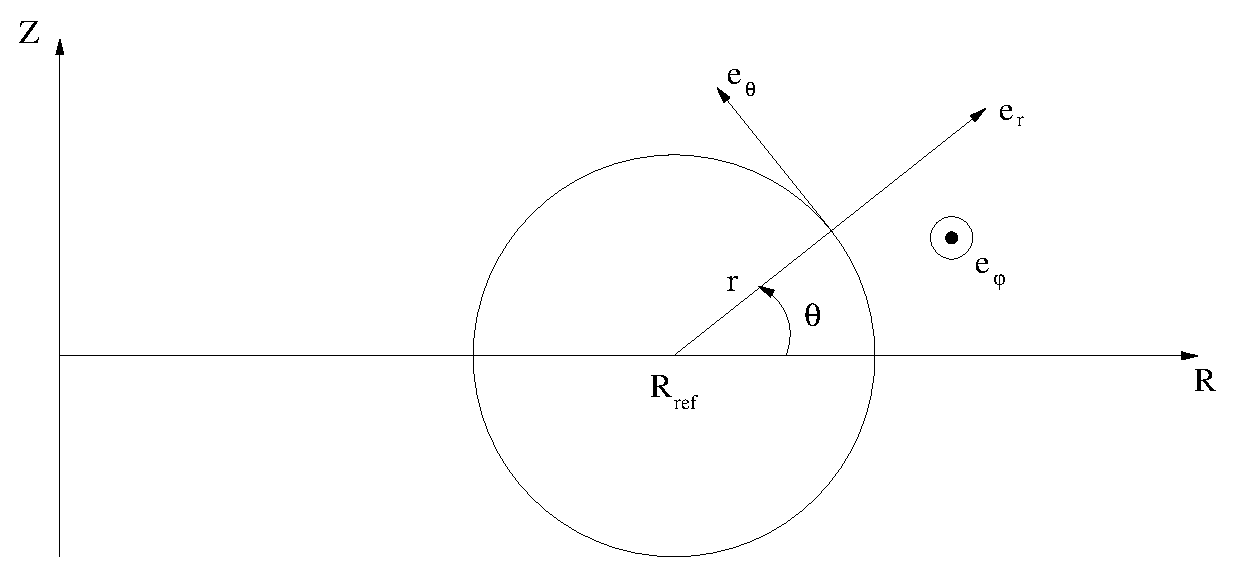
\includegraphics[width=0.6\textwidth]{circFS.eps}
\caption{Circular flux surface centred on $R=R\ind{ref}$, $Z=0$ and $(r,\theta,\varphi)$ coordinates.\label{circFS}}
\end{center}
\end{figure}

In this section, unless explicitly denoted by a $N$ subscript, the various quantities are not normalised. The starting assumption of the model is that the flux surfaces are circular and concentric
with the poloidal flux being a function of the radial coordinate only $\Psi=\Psi(r)$, see
figure~\ref{circFS}. This is a valid assumption in the case of small $\epsilon$ and small $\beta$. It simply means that the terms of order $\epsilon^2$ are neglected and that the Shafranov shift is
considered to be of order $\epsilon^2$.
For simplicity, the various terms are not expanded in $\epsilon$ in the following calculation, but one has to remember that the results are only valid up to order $\epsilon$.
The second assumption of the model is that the radial derivative of the poloidal flux is given by:
\begin{equation}
 \pd{\Psi}{r}=\frac{r B\ind{ref}}{\bar{q}}
\end{equation}
where $B\ind{ref}$ is the value of the magnetic field at $R\ind{ref}$ taken to be the major radius of the magnetic axis (i.e. the centre of the flux surfaces) and $\bar{q}>0$ is a parameter directly
related to the safety factor $q$. The flux surfaces are parametrised by $R=R\ind{ref}+r \cos \theta$ and $Z=r \sin\theta$ in the $(r,\theta,\varphi)$ coordinates system. The inverse aspect ratio is
defined as $\epsilon=r/R\ind{ref}$ and it might be worth reminding that:
\begin{equation}
 \nabla \epsilon = \frac{1}{R\ind{ref}} \mathbf{e_r}, \qquad \nabla \theta = \frac{1}{\epsilon R\ind{ref}}\mathbf{e_\theta}, \qquad \nabla \varphi = \frac{1}{R} \mathbf{e_\varphi}
\end{equation}
Another useful quantity is the Jacobian of the $(\Psi,\theta,\varphi)$ coordinates system which can be expressed as
\begin{equation}
 {J_{\Psi\theta\varphi}}^{-1}=\nabla\Psi\times\nabla\theta\cdot\nabla\varphi=\pd{\Psi}{r}{J_{r\theta\varphi}}^{-1}=\pd{\Psi}{r}\frac{1}{rR}=\frac{B\ind{ref}}{\bar{q}R}
\end{equation}

As usual, the magnetic field is decomposed into its toroidal and poloidal components:
\begin{equation}
 \mathbf{B} = s\ind{B}F(\Psi)\nabla \varphi + s\ind{j} \nabla \varphi \times \nabla \Psi
\end{equation}
One furthermore assumes that $F(\Psi)=R\ind{ref}B\ind{ref}$ and the magnetic field can then be written as
\begin{equation}
 \mathbf{B} = R\ind{ref}B\ind{ref}\left[ s\ind{B} \nabla \varphi + s\ind{j}\frac{1}{\bar{q}}\frac{\epsilon^2}{1+\epsilon\cos\theta}\nabla \theta\right]
\end{equation}
The definition of the safety factor is
\begin{equation}
 q=\frac{1}{2\pi}\int_0^{2\pi}\frac{\mathbf{B}\cdot\nabla\varphi}{\mathbf{B}\cdot\nabla\theta}\,\textrm{d}\theta
\end{equation}
which in the model considered here leads to
\begin{equation}
 q=\frac{1}{2\pi}\int_0^{2\pi}s\ind{B}s\ind{j}J_{\Psi\theta\varphi}\frac{R\ind{ref}B\ind{ref}}{R^2}\,\textrm{d}\theta=s\ind{B}s\ind{j}\frac{\bar{q}}{2\pi}\int_0^{2\pi}
\frac{1}{1+\epsilon\cos\theta}\,\textrm{d}\theta=s\ind{B}s\ind{j}\frac{\bar{q}}{\sqrt{1-\epsilon^2}}
\end{equation}
which makes explicit the relationship between $q$ and $\bar{q}$.

We now have all the ingredients to derive the field aligned coordinates $(\psi,\zeta,s)$. In GKW, $\psi$ is defined to be $\epsilon$ and we will use this notation in the following to avoid possible
confusion with the poloidal flux $\Psi$. The definition of the parallel coordinate $s$ is
\begin{equation}
 s = \int_0^\theta \frac{\textrm{d}\theta}{\mathbf{B}\cdot\nabla\theta} \,\,\Big{/} \int_0^{2\pi} \frac{\textrm{d}\theta}{\mathbf{B}\cdot\nabla\theta}
\end{equation}
So, we first calculate
\begin{equation}
 \int_0^\theta \frac{\textrm{d}\theta}{\mathbf{B}\cdot\nabla\theta} = \int_0^\theta s\ind{j}J_{\Psi\theta\varphi}\,\textrm{d}\theta = s\ind{j}\bar{q}\frac{R\ind{ref}}{B\ind{ref}} \int_0^\theta
[1+\epsilon\cos\theta]\,\textrm{d}\theta = s\ind{j}\bar{q}\frac{R\ind{ref}}{B\ind{ref}} [\theta + \epsilon \sin\theta],
\end{equation}
to get
\begin{equation}
 s=\frac{1}{2\pi}[\theta + \epsilon\sin\theta]
\label{eq:s:def}
\end{equation}
and
\begin{eqnarray}
 \pd{s}{\epsilon} &=& \frac{1}{2\pi}\sin\theta, \\
 \pd{s}{\theta} &=& \frac{1}{2\pi}[1+\epsilon\cos\theta],\\
 \pd{s}{\varphi} &=& 0.
\end{eqnarray}
The definition of the $\zeta$ coordinate is:
\begin{equation}
 \zeta = - \frac{\varphi}{2\pi} + s\ind{B}s\ind{j}\frac{F}{2\pi}\int_0^\theta \frac{J_{\Psi\theta\varphi}}{R^2}\,\textrm{d}\theta 
\end{equation}
which in the ad-hoc circular model gives
\begin{equation}
 \zeta = - \frac{\varphi}{2\pi} + s\ind{B}s\ind{j}\frac{\bar{q}}{2\pi}\int_0^\theta \frac{\textrm{d}\theta}{1+\epsilon\cos\theta}
\end{equation}
Noticing that
\begin{equation}
 \int_0^\theta \frac{\textrm{d}\theta}{1+\epsilon\cos\theta} = \frac{2}{\sqrt{1-\epsilon^2}}\arctan\left[ \sqrt{\frac{1-\epsilon}{1+\epsilon}}\tan \frac{\theta}{2}\right],
\end{equation}
one gets
\begin{equation}
 \zeta = - \frac{\varphi}{2\pi} + s\ind{B}s\ind{j}\frac{|q|}{\pi}\arctan\left[ \sqrt{\frac{1-\epsilon}{1+\epsilon}}\tan \frac{\theta}{2}\right]
 \label{eq:def:zeta}
\end{equation}
and
\begin{eqnarray}
 \pd{\zeta}{\epsilon} &=& s\ind{B}s\ind{j}\frac{|q|}{\epsilon\pi}\left[ \hat{s}\arctan\left[ \sqrt{\frac{1-\epsilon}{1+\epsilon}}\tan \frac{\theta}{2}\right] -
\frac{\epsilon\tan\frac{\theta}{2}}{\sqrt{1-\epsilon^2}\left(1+\epsilon+(1-\epsilon)\tan^2\frac{\theta}{2}\right)} \right], \\
 \pd{\zeta}{\theta} &=& s\ind{B}s\ind{j}\frac{|q|}{2\pi}\frac{\sqrt{1-\epsilon^2}}{1+\epsilon\cos\theta},\\
 \pd{\zeta}{\varphi} &=& -\frac{1}{2\pi}.
\end{eqnarray}
From the decomposition of $\nabla s$ and $\nabla \zeta$ as a function of $\nabla \epsilon$, $\nabla \theta$ and $\nabla\varphi$
\begin{eqnarray}
 \nabla s &=& \pd{s}{\epsilon} \nabla\epsilon +  \pd{s}{\theta} \nabla\theta +  \pd{s}{\varphi} \nabla\varphi \\
 \nabla \zeta &=& \pd{\zeta}{\epsilon} \nabla\epsilon +  \pd{\zeta}{\theta} \nabla\theta +  \pd{\zeta}{\varphi} \nabla\varphi ,
\end{eqnarray}
the calculation of the metric tensor is straightforward:
\begin{eqnarray}
 g^{\epsilon\epsilon}_N &= R\ind{ref}^2 g^{\epsilon\epsilon} &= 1,\\
 g^{\epsilon\zeta}_N &= R\ind{ref}^2 g^{\epsilon\zeta} &= \pd{\zeta}{\epsilon},\\
 g^{\epsilon s}_N &=R\ind{ref}^2 g^{\epsilon s} &= \frac{1}{2\pi}\sin\theta,\\
 g^{\zeta\zeta}_N &= R\ind{ref}^2 g^{\zeta\zeta} &= \left[\pd{\zeta}{\epsilon}\right]^2 + \left[\frac{1}{2\pi}\frac{1}{1+\epsilon\cos\theta} \right]^2
\left[1+\frac{q^2}{\epsilon^2}(1-\epsilon^2)\right]\\
 g^{\zeta s}_N &= R\ind{ref}^2 g^{\zeta s} &= \frac{\sin\theta}{2\pi}\pd{\zeta}{\epsilon} + s\ind{B}s\ind{j}\frac{|q|}{(2\pi\epsilon)^2}\sqrt{1-\epsilon^2}\\
 g^{s s}_N &= R\ind{ref}^2 g^{s s} &= \frac{1}{4\pi^2}\left[ 1 + \frac{2}{\epsilon}\cos\theta + \frac{1}{\epsilon^2}\right].
\end{eqnarray}
To calculate the other metric elements one needs the norm of the magnetic field
\begin{equation}
 B=\sqrt{\mathbf{B}\cdot\mathbf{B}}=\frac{B\ind{ref}}{1+\epsilon\cos\theta}\left[ 1+ \frac{1}{q^2}\frac{\epsilon^2}{1-\epsilon^2} \right]^{1/2}
\end{equation}
and its gradient
\begin{equation}
 \nabla B = \pd{B}{\epsilon} \nabla \epsilon + \pd{B}{\theta} \nabla \theta
\end{equation}
which involves
\begin{eqnarray}
 \pd{B}{\epsilon} &=&  \left[ -\frac{\cos\theta}{1+\epsilon\cos\theta} + \frac{\epsilon}{\epsilon^2+q^2(1-\epsilon^2)}(1-\hat{s}+\frac{\epsilon^2}{1-\epsilon^2})\right]B\\
 \pd{B}{\theta} &=& \frac{\epsilon\sin\theta}{1+\epsilon\cos\theta}B
\end{eqnarray}
From the definition 
\begin{equation}
 \mathcal{D}^\alpha_N = \frac{R\ind{ref}^2}{B^2B_N}\mathbf{B}\times\nabla B \cdot \nabla x^\alpha
\end{equation}
and some straightforward algebra (which has to be understood as ``I am by far too lazy to write down all the steps in \LaTeX'') we get the components of the tensor related to the curvature and
$\nabla B$ drift:
\begin{eqnarray}
 \mathcal{D}^{\epsilon}_N &=& -s\ind{B} \sin\theta \frac{1}{1+\frac{1}{q^2}\frac{\epsilon^2}{1-\epsilon^2}} \\
 \mathcal{D}^{\zeta}_N &=& \left[\frac{s\ind{j}}{2\pi} \frac{1}{B}\pd{B}{
\epsilon}\left(\frac{|q|\sqrt{1-\epsilon^2}}{\epsilon}+\frac{\epsilon}{|q|\sqrt{1-\epsilon^2}}\right)-s\ind{B}\pd{\zeta}{\epsilon}\sin\theta \right]
\frac{1}{1+\frac{1}{q^2}\frac{\epsilon^2}{1-\epsilon^2}}\\
 \mathcal{D}^{s}_N &=& \frac{s\ind{B}}{2\pi}\left[\frac{1}{\epsilon B}\pd{B}{\epsilon}(1+\epsilon\cos\theta)^2 -\sin^2\theta\right]
\frac{1}{1+\frac{1}{q^2}\frac{\epsilon^2}{1-\epsilon^2}}\\
\end{eqnarray}
The tensor related to the $\mathbf{E}\times\mathbf{B}$ drift can be obtained from the metric tensor elements:
\begin{equation}
 \mathcal{E}^{\alpha\beta}_N = s\ind{j}\frac{\pi R\ind{ref}^2}{BB_N}\pd{\Psi}{\epsilon}(g^{\alpha\epsilon} g^{\beta\zeta} - g^{\alpha\zeta} g^{\beta\epsilon})
\end{equation}
which for the ad-hoc model gives:
\begin{equation}
 \mathcal{E}^{\alpha\beta}_N = s\ind{j}\frac{\pi }{B_N^2}\frac{\epsilon}{|q|\sqrt{1-\epsilon^2}}(g^{\alpha\epsilon}_N g^{\beta\zeta}_N - g^{\alpha\zeta}_N g^{\beta\epsilon}_N)
\end{equation}
We the calculate the tensor related to the parallel derivative 
\begin{equation}
 \mathcal{F}_N = R\ind{ref} \frac{\mathbf{B}\cdot\nabla s}{B} = \frac{s\ind{j}}{2\pi |q| B_N}\frac{1}{\sqrt{1-\epsilon^2}}
\end{equation}
and the tensor related to the trapping
\begin{equation}
 \mathcal{G}_N = \frac{R\ind{ref}\mathbf{B}\cdot\nabla B}{B^2} = s\ind{j}\frac{\epsilon B_N \sin \theta}{|q|\sqrt{1-\epsilon^2}}\frac{1}{1+\frac{1}{q^2}\frac{\epsilon^2}{1-\epsilon^2}}.
\end{equation}
For the tensor related to the Coriolis drift
\begin{equation}
 \mathcal{H}^\alpha_N=\frac{R\ind{ref}}{B_N\Omega}\mathbf{\Omega}_\perp\cdot\nabla x^\alpha,
\end{equation}
we first decompose $\mathbf{\Omega}$ as
\begin{equation}
 \mathbf{\Omega} = -s\ind{B}\Omega\nabla Z = -s\ind{B}R\ind{ref}\Omega\left[ \sin\theta \nabla \epsilon + \epsilon \cos \theta \nabla \theta\right]
\end{equation}
to get
\begin{equation}
 \mathbf{\Omega}\cdot\mathbf{b} = -s\ind{B}s\ind{j}\Omega\frac{\epsilon\cos\theta}{|q|\sqrt{1-\epsilon^2}}\frac{R\ind{ref}B\ind{ref}}{RB} 
\end{equation}
and finally obtain
\begin{eqnarray}
 \mathcal{H}^\epsilon_N &=& -\frac{s\ind{B}}{B_N}\sin\theta \\
 \mathcal{H}^\zeta_N &=& -\frac{s\ind{B}}{B_N}\sin\theta\pd{\zeta}{\epsilon} -
                         \frac{s\ind{j}|q|\cos\theta}{2\pi\epsilon B_N}\frac{\sqrt{1-\epsilon^2}}{1+\epsilon\cos\theta}\\
 \mathcal{H}^s_N &=& -\frac{s\ind{B}}{2\pi B_N}\sin^2\theta + \frac{s\ind{B}}{2\pi B_N}(1+\epsilon\cos\theta)\left[ -\frac{\cos\theta}{\epsilon} + \frac{\epsilon\cos\theta}{q^2(1-\epsilon^2)}
\frac{1}{1+\frac{1}{q^2}\frac{\epsilon^2}{1-\epsilon^2}}\right].
\end{eqnarray}
Using
\begin{equation}
 \nabla R = R\ind{ref} \left[\cos\theta \nabla \epsilon -\epsilon\sin\theta\nabla\theta \right] 
\end{equation}
the tensor related to the centrifugal drift, can be expressed as
\begin{equation}
 \mathcal{I}^\alpha_N = s\ind{j}\frac{2\pi}{B_N^2}\frac{\epsilon(1+\epsilon\cos\theta)}{|q|\sqrt{1-\epsilon^2}}\left[g^{\epsilon\alpha}_N\left[\cos\theta\pd{\zeta}{\epsilon} -
s\ind{B}s\ind{j}\frac{|q|}{2\pi\epsilon}\frac{\sin\theta\sqrt{1-\epsilon^2}}{1+\epsilon\cos\theta}\right] -g^{\zeta\alpha}_N\cos\theta\right]
\end{equation}
We also have
\begin{equation}
 {\cal M} = {1 \over q \sqrt{1-\epsilon^2}}\left(1-{\epsilon \over 1-\epsilon^2}-{\hat s \over q}\right).
\end{equation}
Finally, the elements used to calculate the centrifugal potential are 
\begin{equation}
 \mathcal{J}_N= (1+\epsilon\cos\theta)^2-\frac{R_0^2}{R\ind{ref}^2} \qquad \mathcal{K}_N=\pd{\mathcal{J}_N}{
\epsilon} \biggr |_s =2(\cos\theta+\epsilon)-{\cal L}_N
\end{equation}
where the transformation between partial deriviatives at constant $\theta$ and $s$ gives
\begin{equation}
\frac{1}{R\ind{ref}} \pd{R}{\epsilon} \biggr |_s= \cos(\theta) + \frac{\epsilon \sin^2(\theta)}{1+\epsilon \cos(\theta)}
\end{equation}
which has been used to calculate ${\cal K}$.
The two choices for $R_0$ (magnetic axis value or $R(s=0)$) give
\begin{equation}
R_0=R\ind{ref} \Rightarrow {\cal L}_N=0, \quad  
R_0=(1+\epsilon)R\ind{ref} \Rightarrow {\cal L}_N =2(1+\epsilon)
\end{equation}
respectively.

% \subsection{Shifted circular surface geometry} 
% (NOT IMPLEMENTED, NOT CONSISTENT WITH OTHER SECTIONS - not normalised, definitions of Rref and r0 differ)\\
% 
% The shifted circular surface geometry is defined in the ($R,Z$) plane (using cylindrical coordinates
% $(R,\phi,z)$. 
% \begin{equation} 
% R = r \cos \theta + \Delta(r) + R_0 \qquad {\rm with} \qquad \Delta(0) = 0 
% \end{equation}
% \begin{equation} 
% Z = r \sin \theta
% \end{equation}
% Surfaces of constant $r$ are assumed to be flux surfaces. One can confusingly define two major 
% radii. One is the radius of the magnetic axis $R_0$, and one is the major radius of the centre 
% of the surface $R_c$ 
% \begin{equation} 
% R_c = (R(\theta =0) + R(\theta = \pi) )/2 = R_0 + \Delta(r) 
% \end{equation}
% Since the first one is a constant while $R_c$ depends on $r$, we will choose to normalise all 
% the radii with $R_0$, i.e. 
% \begin{equation} 
% R_{\rm ref} = R_0
% \end{equation}
% The normalised radial coordinate then is 
% \begin{equation} 
% \psi = r / R_0 = \epsilon
% \end{equation}
% and we will define a normalised major radius that gives the centre of the surface as 
% \begin{equation} 
% R_{cN} = 1 + {\Delta (r) \over R_0} 
% \end{equation}
% 
% From the equations above one can work out
% \begin{equation} 
%   \bbmatrix
%     \nabla r      \\
%     \nabla \theta
%   \ebmatrix
%   = {1\over r (1 + \Delta^\prime \cos \theta)} 
%   \bbmatrix
%     r \cos \theta & r \sin \theta \\
%     - \sin \theta & \Delta^\prime + \cos \theta
%    \ebmatrix
%    \bbmatrix
%      \nabla R \\
% 	 \nabla Z
%    \ebmatrix 
% \end{equation}
% where 
% \begin{equation}
%   \Delta^\prime = {{\rm d} \Delta \over {\rm d} r} 
% \end{equation}
% The poloidal magnetic field can be written as 
% \begin{equation} 
% {\bf B}_p = B_p {{\bf e}_\theta \over \vert {\bf e}_\theta \vert} \qquad 
% {\bf e}_\theta = \pd{{\bf x}}{\theta} =
% \bbmatrix
%   -r \sin \theta \\
%    r \cos \theta
% \ebmatrix  
% \end{equation} 
% From which it folows that 
% \begin{equation} 
% {\bf e}_\theta \cdot \nabla \theta = 1 \qquad {\bf B} \cdot \nabla \theta = B_p / r 
% \end{equation} 
% From flux conservation 
% \begin{equation} 
% R B_p {\rm d}l_\perp = {R B_p \over \vert \nabla r \vert } {\rm d} r = {\rm constant} 
% \end{equation}
% It follows that  
% \begin{equation} 
% {B_p \over B_p(\pi/2)} = {R_{cN}(\psi) \over (1 + \Delta^\prime(\psi) \cos \theta) (R_{cN}(\psi) + \psi \cos \theta)}
% \end{equation}
% The integral to obtain $s$ and $B^s$ can be easily performed 
% \begin{equation} 
% B^s = {B_p(\pi/2)\over 2 \pi ( 1 + \psi \Delta^\prime / 2 R_{Nc} )}
% \end{equation}
% \begin{equation} 
% s = {\theta \over 2 \pi} + {2 \psi \sin \theta + 2 \Delta^\prime R_{cn} \sin \theta + \Delta^\prime \psi 
% \cos \theta \sin \theta \over 4 \pi R_{cn} ( 1 + \Delta^\prime \psi / 2 R_{cn})}
% \end{equation}
% After some manipulations also the flux surface average of $1/R^2$ can be expressed as 
% \begin{equation} 
% \biggl \langle {1 \over R^2} \biggr \rangle = {1\over R_0^2} {1 \over R_{cN} + \psi \Delta^\prime / 2} 
% \biggl [ {1 - \Delta^\prime \over \sqrt{R_{cN}^2 - \psi^2} } + {\Delta^\prime \over \psi} \biggr ] 
% \end{equation}

\subsection{Miller parametrisation}
Miller parametrisation of the flux surface shape is a good compromise between the flexibility of the circ geometry and the precision of an equilibrium obtained from the solutin of the Grad-Shafranov equation.
In this section the Miller parametrisation first done in \cite{MIL98} is described. Then the derivation of the metric tensor in GKW coordinate system ($\psi,\zeta,s$) and the derivatives of the magnetic field are shown using the implementation method of \cite{CAN09}. \\
To avoid any confusion between the poloidal magnetic flux and the radial coordinate the latter will be called $r$ through the entire section.  For the miller geometry, $R_{\rm ref} = (R_{\rm max} + R_{\rm min})/2 $ which is the geometric axis of the flux surface in question.

\subsubsection{Parametrisation (Input List)}
The following parameters are used to describe a magnetic flux surface in (R,Z) plane : $\kappa$ (elongation), $\delta$ (triangularity), $\zeta$ (squareness), $R_{\rm mil}$, $Z_{\rm mil}$, and their radial derivatives $s_\kappa, s_\delta ($definition of$ \cite{MIL98}), s_\zeta, {\mathrm{d} R_{
\rm mil} \over \mathrm{d}r}$, ${\mathrm{d}Z_{\rm mil} \over \mathrm{d}r}$ defined such that:  
\begin{equation}
s_\kappa  =  {r \over \kappa}{\mathrm{d}\kappa \over \mathrm{d}r}, \qquad
s_\delta  =  r{{\mathrm{d}\delta \over \mathrm{d}r} \over \sqrt{1-\delta^2}}, \qquad
s_\zeta  = r{\mathrm{d}\zeta \over \mathrm{d}r}
\end{equation}
Parameters such as ${\mathrm{d} p \over \mathrm{d} \Psi}$ (pressure gradient), q (safety factor), $\hat s$ (magnetic shear) and $\epsilon$ (aspect ratio $= {r \over R_{
\rm mil}}$) are also used.
Flux surfaces geometry are then given by :
\begin{eqnarray}
R &=& R_{\rm mil} + r \cos{(\theta + \arcsin \delta \sin \theta)} \\
Z &=& Z_{\rm mil} + r \kappa \sin{(\theta + \zeta \sin{2\theta})}
\end{eqnarray}
and the radial derivatives of R and Z by :
\begin{eqnarray}
\pd{ R}{r} &=& {\mathrm{d}R_{\rm mil} \over \mathrm{d}r} + \cos{(\theta + \arcsin \delta \sin \theta)} - s_\delta \sin{\theta} \sin{(\theta + \arcsin \delta \sin \theta)} \\
\pd{ Z}{r} &=& {\mathrm{d}Z_{\rm mil} \over \mathrm{d}r} + \kappa \sin{(\theta + \zeta \sin{2\theta})} + \kappa s_\kappa \sin{(\theta + \zeta \sin{2\theta})} + \kappa s_\zeta \sin{(2\theta)} \cos{(\theta + \zeta \sin{2\theta})}
\end{eqnarray}
Examples how the parameters affect the cross section of a flux surface can be
seen in Fig.~\ref{fig:examplemillergeom}.
\begin{figure}
  \begin{center}
    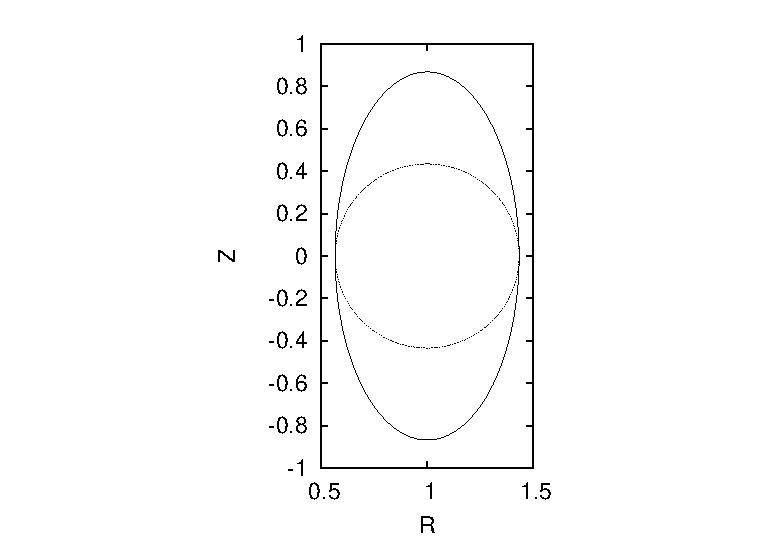
\includegraphics[width=0.49\textwidth]{millergeomkappa}
    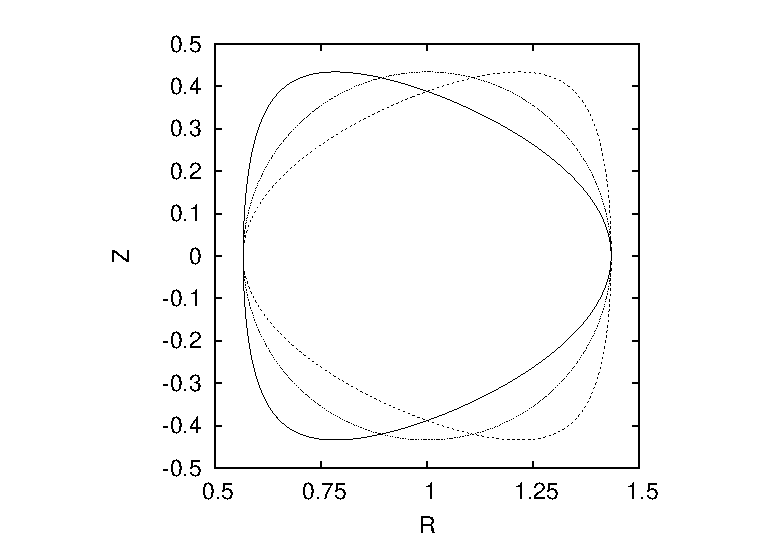
\includegraphics[width=0.49\textwidth]{millergeomdelta}
    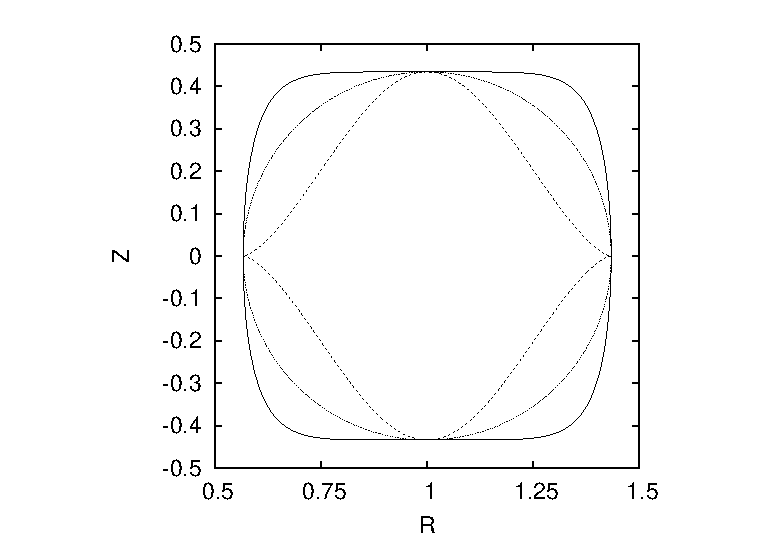
\includegraphics[width=0.49\textwidth]{millergeomzeta}
    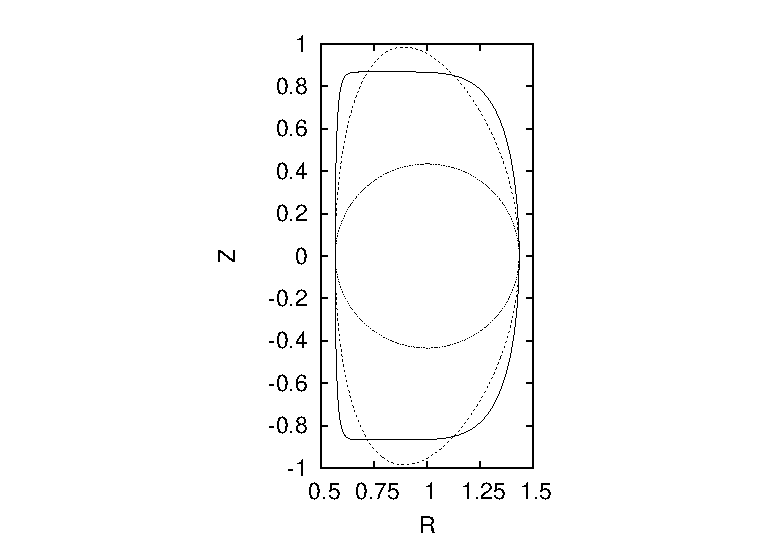
\includegraphics[width=0.49\textwidth]{millergeomall}
    \caption[Examples Miller geometry]{\label{fig:examplemillergeom}
    Examples for the effects of $\kappa$, $\delta$ and $\zeta$ in Miller
    geometry. In all plots shown in this drawing, the dashed line is a circular flux surface.
    Top left: $\kappa=2.0$, $\delta=\zeta=0.0$. Top right: The
    full/dashed line has $\delta=\pm 0.5$, $\kappa=1.0$ and $\zeta=0.0$. Bottom
    left: The full/dashed line has $\zeta=\pm 0.5$, $\kappa=1$ $\delta=0.0$.
    Bottom right: The full line has $\kappa=2$, $\delta=0.5$ and $\zeta=0.5$.
    The dashed line is an example taken from an actual experiment
    with $\kappa=2.25$, $\delta=0.25$, $\zeta=-0.016$.}
  \end{center}
\end{figure}
The pressure gradient can be computed from different parameters through the input \textit{gradp\_type}.
The input list is also defined in the file \doc{input.dat.sample}.

The normalisation is made such that:
\begin{eqnarray}
R_N &=& 1 + \epsilon \cos (\theta + \arcsin \delta \sin \theta) \\
F_N &=& 1
\end{eqnarray}
We have then $R_{\rm ref} = R_{\rm mil}$ and $B_{\rm ref} = B_t(R_{\rm mil})$. \\
The normalisation for the plasma pressure gradient is given here using :
\begin{equation}
\left({\mathrm{d} p \over \mathrm{d} \Psi}\right)_N = {2 \mu_0 R_{\rm ref}^2\over B_{\rm ref}} {\mathrm{d} p \over \mathrm{d} \Psi}
\end{equation}
The normalised pressure gradient used in the code can be given by :
\begin{eqnarray}
\left({\mathrm{d} p \over \mathrm{d} \Psi}\right)_N &=& - \alpha {\left(2\pi^2\right) \over \left(\partial_{\Psi}V\right)_N } \left({V_N \over 2\pi ^2}\right)^{-1/2}\\
\left({\mathrm{d} p \over \mathrm{d} \Psi}\right)_N &=& {\alpha_{MHD}\over \epsilon ^2}\left({\mathrm{d} \Psi \over \mathrm{d} \epsilon}\right)_N \\
\left({\mathrm{d} p \over \mathrm{d} \Psi}\right)_N &=& {\beta ' \over 2 {\mathrm{d} \Psi_N \over \mathrm{d} \epsilon}}
\end{eqnarray}
with $\alpha$ taken from equation 42 in \cite{MIL98}, $\alpha_{MHD}$ from equation 141 \cite{CAN09} and $\beta '$ is defined in section \ref{Sec:betabetapr}. \\
For centrifugal effects on the pressure gradient go to equation \ref{eq:rota}. \\
The equations used below are not normalised however they are in the code. \\
In the coordinate system $(r,\theta,\varphi)$ where the magnetic flux surfaces are described, the elements of the metric tensor are :
\begin{eqnarray}
g_{rr} &=& \left(\pd{ R}{r}\right)^2 + \left(\pd{ Z}{r}\right)^2, \\
g_{r \theta} &=& \pd{ R}{r}\pd{ R}{\theta} + \pd{ Z}{r}\pd{ Z}{\theta} \\
g_{\theta \theta} &=& \left(\pd{ R}{\theta}\right)^2 + \left(\pd{ Z}{\theta}\right)^2, \\
g_{\varphi \varphi} &=& R^2
\end{eqnarray}
The contravariant metric tensor, used to calculate the contravariant metric tensor of the GKW basis, is deduced from the relation $g_{ij} \cdot g^{ij} = I$ with I the identity matrix.
\subsubsection{Mercier-Luc coordinate system}
An expansion of the poloidal flux $\Psi$ is needed. A coordinate system (introduced by Mercier-Luc) is defined such that the expansion is easy to use (orthogonal system ($\rho,l,\varphi$)).
\begin{figure}[h]
\begin{center}
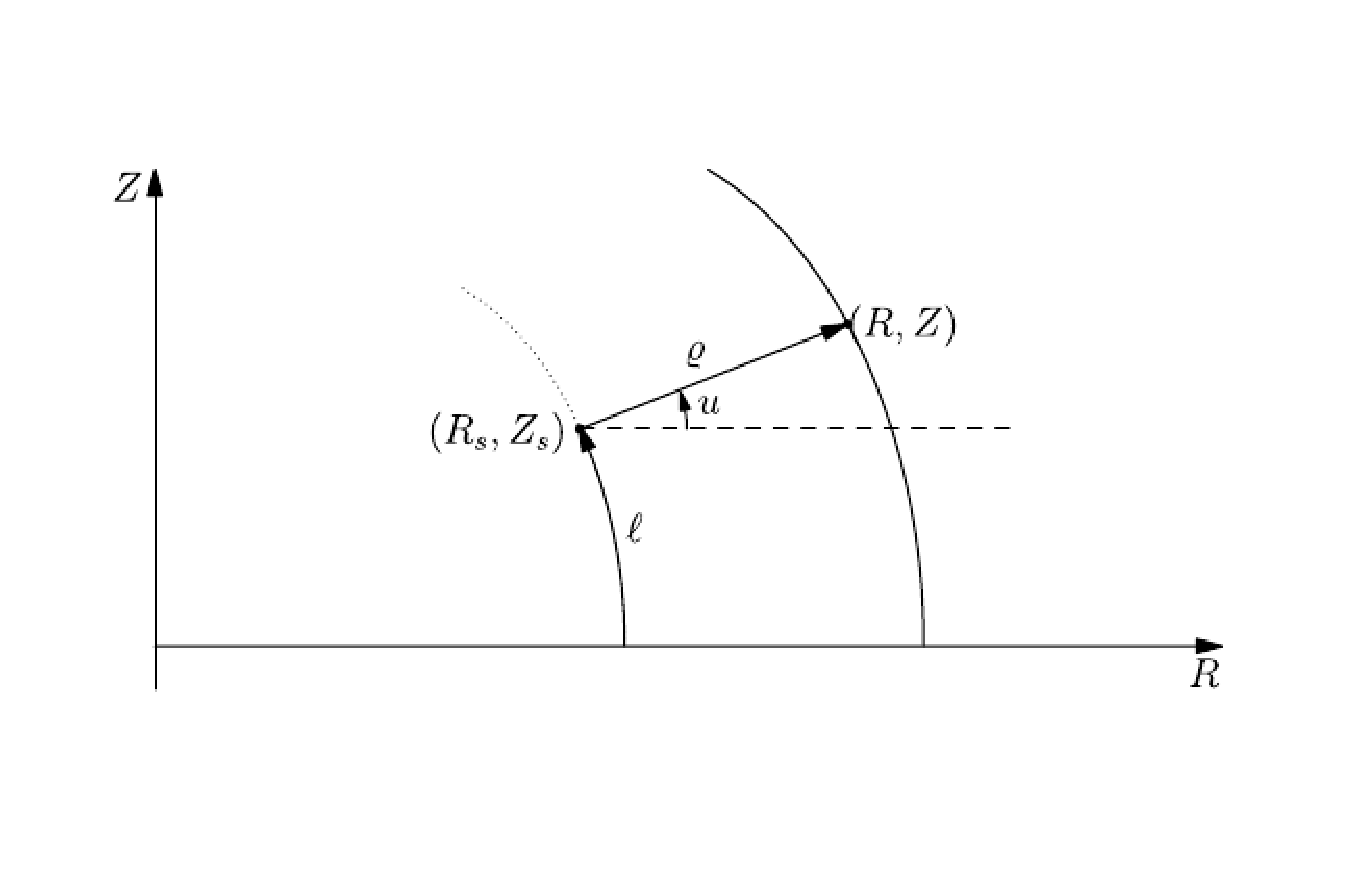
\includegraphics[width=0.6\textwidth]{mercier-luc.eps}
\caption{Mercier-Luc coordinate system.\label{merc-luc}...from \cite{CAN09}}
\end{center}
\end{figure}
In addition to the plasma shape, 
the gradient of the plasma pressure must also be specified, which in GKW can be done independently for the geometry, or by coupling to $\beta^\prime$.

\begin{eqnarray}
\Psi &=& \Psi_s + \rho \Psi_1 + \rho^2 \Psi_2 \\
R &=& R_s + \rho \cos{u} \\
Z &=& Z_s + \rho \sin{u}
\end{eqnarray}
with 
\begin{eqnarray}
\cos u &=& \pd{ Z_s}{l} \\
\sin u &=& - \pd{ R_s}{l}
\end{eqnarray}
where the subscript s means the value on the surface of consideration. \\
The metric elements are: 
\begin{eqnarray}
g_{\rho \rho} &=& 1 \\
g_{ll} &=& \left(1 + {\rho \over r_c} \right) \\
g_{\varphi \varphi} &=& R^2
\end{eqnarray}
The Jacobian is then:
\begin{equation}
J_\rho = R \left(1 + {\rho \over r_c}\right) 
\end{equation}
with $r_c$ being the curvature radius :
\begin{equation}
r_c = g_{\theta \theta}^{3/2} \left(\pd{ R}{\theta}\pdd{Z}{ \theta}-\pd{ Z}{\theta}\pdd{R}{\theta}\right)^{-1} 
\end{equation}
To switch from $(\rho,l,\varphi)$ to $(r,\theta,\varphi)$ the following relations are important (all quantities are taken on the flux surface)  :
\begin{eqnarray}
\pd{ \rho}{r} &=& \cos u \pd{ R}{r} + \sin u \pd{ Z}{r} \\
\pd{ l}{r} &=& \cos u \pd{ Z}{r} - \sin u \pd{ R}{r} \\
\pd{ \rho}{\theta} &=& 0 \\
\pd{ l}{\theta} &=& \sqrt{g_{\theta \theta}}
\end{eqnarray}
From the definition of the poloidal magnetic field:
\begin{equation}
B_p^2 = |\nabla \varphi|^2|\nabla \Psi|^2 = {\Psi_1 ^2 \over R_s ^2 }
\end{equation}
one finds
\begin{equation}
\Psi_1 = R_s B_{ps}
\end{equation}
$\Psi_2$ is obtained from the Grad-Shafranov equation for the expansion of $\Psi$:
\begin{equation}
R \nabla \cdot{\nabla \Psi \over R^2} = -\mu_0 R^2 p'(\Psi) - FF'(\Psi)
\end{equation}
with ' corresponding to the derivative toward the poloidal magnetic flux.
One can easily obtain: 
\begin{equation}
\Psi_2 = {1 \over 2}\left(B_p \cos u - {B_p R \over r_c} - \mu_0 R^2 p' - FF'\right)
\end{equation}
From this point we see that we have other parameters : $F$ (see the normalisation section), $F'$, $p'$, ${d \Psi \over dr}$ that we need to link to our first set of parameters.
The relation for $F'$ will be expressed later (it is not trivial).
\subsubsection{Relations for $p'$ and ${d\Psi \over dr}$}
${d\Psi \over dr}$ is obtained from the definition of $q$:
\begin{equation}
q = {1 \over 2 \pi} \int_0^{2\pi} {{{\bf B} \cdot \nabla \varphi \over {\bf B} \cdot \nabla \theta}\mathrm{d}\theta} 
\end{equation}
with 
\begin{equation}
{\bf B} = s_B F \nabla \varphi + s_J \nabla \varphi \times \nabla \Psi
\end{equation}
It follows : 
\begin{equation}
q = s_B s_J{F \over 2 \pi {\mathrm{d}\Psi \over \mathrm{d}r}} \int_0^{2\pi}{{J_r \over R^2}\mathrm{d}\theta}
\end{equation}
yields 
\begin{equation}
{\mathrm{d}\Psi \over \mathrm{d}r} = s_B s_J{F \over 2 \pi q} \int_0^{2\pi}{{J_r \over R^2}\mathrm{d}\theta}
\end{equation}
Numerical integrals are implemented using Simpson's method. \\
$p'$ is given from the relation in \cite{MIL98}:
\begin{equation}
\alpha = -{2\pd{ V}{\Psi} \over (2 \pi)^2}\left({V \over 2 \pi^2 R_{
\rm mil}}\right)^{1/2} \mu_0 p^\prime
\end{equation}
V is the volume defined by the magnetic flux surface :
\begin{equation}
V = 2 \pi S R_G
\end{equation}
with
\begin{eqnarray}
R_G &=& {\int_0^{2\pi} {R \sqrt{(\pd{ R}{\theta})^2 + (\pd{ Z}{\theta})^2} \mathrm{d}\theta} \over \int_0^{2\pi} {\sqrt{(\pd{ R}{\theta})^2 + (\pd{ Z}{\theta})^2} \mathrm{d}\theta}} \\
S &=& \int_0^{2\pi} {Z\pd{ R}{\theta}}
\end{eqnarray}
$\pd{ V}{\Psi}$ can easily be defined analytically by differentiating towards $r$ and using ${\mathrm{d}\Psi \over \mathrm{d}r}$ \\
\\
 
\subsubsection{Effect of toroidal rotation on the magnetic equilibrium}
Force balance equation for species a:

\begin{align}
m_an_a\left(\pd{}{t}+V_a\cdot \nabla \right)V_a = -\nabla p_a - \nabla \cdot \pi_a + e_a n_a\left(E+V_a\times B\right)+R_a
\end{align}

Viscosity $\nabla \cdot \pi_a$ and friction $R_a$ are being neglected. \\
A two species model with singly (for now) charged ions is considered (trace species can be added but won't affect the magnetic equilibrium: $m_tn_t \ll m_in_i$, i being the main ion species). Using $m_e \ll m_i$ and taking the dot product of force balance equation with $\mathbf b$, one obtains:

\begin{align}
n_e &= n_{R_0,e}\exp{\left({e \Phi \over T_e}\right)} \\
n_i &= n_{R_0,i}\exp{\left({-e \Phi \over T_i }+ {m_i\Omega^2(R^2 - R_0^2)\over 2T_i}\right)}
\end{align}

$T_i$ is supposed to be a flux function (might not be always the case \cite{THYA06}) \\
Using Quasineutrality and $T_e \sim T_i$:
\begin{align}
e\phi = {T_e \over T_e + T_i}{m_i \over T_i}{1 \over 2}\Omega^2\left(R^2-R_0^2\right)
\end{align}

The total pressure is then:
\begin{align}
p = Tn\exp{\left({m_i\Omega^2 \over 2 T}(R^2-R_0^2)\right)}
\end{align}

with $T = T_e + T_i$.\\
Furthermore the Grad-Shafranov is modified ($\Psi$ and $R^2$ are regarded as independant variables \cite{THYA06}):
\begin{equation}
R^2 \nabla \cdot \left({\nabla \Psi \over R^2}\right) = -\mu_0 R^2 \pd{ p \left(\Psi,R^2\right)}{\Psi} - FF'
\end{equation}

In normalised units one gets 
\begin{align} \label{eq:rota}
\left(\pd{ p}{\Psi}\right)_N &= {1 \over 2}\left[\beta' + \beta_{ref} n_Rm_{R,i}
\left(\left(R_N^2-R_0^2\right)\left(-2u_N' \Omega + {T_{R,e}{R\over L_{T_e}} + T_{R,i}{R \over L_{T_i}}\over \left(T_{R,e}+T_{R,i}\right)}\right)\right.\right. \nonumber \\
&\left.\left.\left. -R_0\pd{ R_0}{\epsilon}\Omega^2\right)\right)\right]\left({d \psi \over d \Psi}\right)_N\exp{\left({m_{R,i}\Omega_N^2 \over \left(T_{R,e}+T_{R,i}\right)}\left(R_N^2-R_0^2\right)\right)}
\end{align}

From this definition, it enters normalised Grad-Shafranov equation through:
\begin{equation}
\left(R^2 \nabla \cdot \left({\nabla \Psi \over R^2}\right)\right)_N = - R_N^2 \left(\pd{ p \left(\Psi,R^2\right)}{\Psi}\right)_N - F_NF_N'
\end{equation}


$\beta'$ is given in SPCGENERAL. $\beta_{ref}$ can be taken from SPCGENERAL but can also be given using the GEOM parameter \textit{beta\_rota\_miller\_type = 'geom'} and specifying the value in \textit{beta\_rota\_miller}. The other parameters are taken from SPECIES and ROTATION namelists.


\textbf{Modification of the curvature drift}

The magnetic curvature can be recast as:
\begin{eqnarray}
\kappa &=& - \mathbf b \times \left(\nabla \times {\mathbf B \over B} \right) \\
\kappa &=& - {1 \over B} \mathbf{b}\times \left(\nabla \times \mathbf{B}\right) - \mathbf{b} \times \left[\nabla\left({1 \over B}\right) \times \mathbf{B}\right] \\
\kappa &=& {\mu_0 J\times B \over B^2}+{\nabla_\bot \mathbf B \over B} \\
\end{eqnarray}

We will now only consider:
\begin{align}
\kappa_1 = \mu_0 {J \times B \over B^2}
\end{align}
since the term $\nabla_\bot B$ is not modified by rotation.\\

Without rotation 
\begin{align}
J\times B = \nabla p
\end{align}
which leads to the $\beta'$ correction.

For strong toroidal rotation one obtains for a two fluid model with singly charged ions:

\begin{align}
J\times B = -m_in_iR\Omega^2\nabla R + \pd{ p}{\Psi} {d \Psi \over d \psi}\nabla \psi + \pd{ p}{R^2} \nabla R^2
\end{align}

The curvature enters Vlasov equation through
\begin{align}
\left(\kappa_1 \times \nabla f\right)\cdot \mathbf{b} = {\mu_0 \over B^2}\left[\left(m_in_i\Omega ^2-2\pd{ p}{R^2}\right) \left(Bs_B\pd{ f}{x_\alpha}\mathcal{I}^\alpha\right)+2\pd{ p}{\Psi}{d \Psi \over d \psi} \pd{ f}{x_\beta} \mathcal{E}^{\psi \beta}\right]
\end{align}

\subsubsection{Determination of $\nabla s$}
We start from the expression of the magnetic field to express the contravariant component $B^s$ in the coordinate system $(\Psi,l,\varphi)$.
\begin{eqnarray}
B^s(\Psi) &=& B \cdot \nabla s \\
&=& B \cdot \nabla l \pd{ s}{l} \\
\pd{ s}{l} &=& B^s {1 \over B \cdot \nabla l}
\end{eqnarray}
Furthermore : 
\begin{equation}
\int_0^L {\pd{ s}{l'}\mathrm{d}l'} = 1 = B^s \int_0^L {{1 \over B \cdot \nabla l'}\mathrm{d}l'}
\end{equation}
with L being the arclength corresponding to $\theta = 2 \pi$.
Hence
\begin{equation}
B^s = {1 \over \int_0^L {{1 \over B \cdot \nabla l'}\mathrm{d}l'}}
\end{equation}
One gets the expression of $s$ in this basis:
\begin{equation}
s = B^s \int_0^l {{1 \over B \cdot \nabla l'}\mathrm{d}l'}
\end{equation}
Using the expansion of the magnetic flux:
\begin{eqnarray}
B \cdot \nabla l &=& s_B F\nabla \varphi \cdot \nabla l + s_j \nabla \varphi \times \left[(\Psi_1 + 2 \rho \Psi_2)\nabla \rho + \rho \pd{ \Psi_1}{l} \nabla l\right] \cdot \nabla l \\
B \cdot \nabla l &=& s_j {\Psi_1 + 2 \rho \Psi_2 \over J_\rho} \\
B \cdot \nabla l &=& s_j {\Psi_1 + 2 \rho \Psi_2 \over (R_s + \rho \cos u)(1 + {\rho \over r_c})}
\end{eqnarray}
Then 
\begin{equation}
{1 \over B \cdot \nabla l} = {s_j \over \Psi_1} \left[R_s + \rho \left(\cos u + {R_s \over r_c} - 2 R_s {\Psi2 \over \Psi1}\right)\right]
\end{equation}
One can write $\nabla s$ as
\begin{equation}
\nabla s = \pd{ s}{\Psi} \nabla \Psi + \pd{ s}{l} \nabla l
\end{equation}
We need then to determine $\pd{ s}{\Psi}$. Using the Mercier-Luc expansion of $\Psi$ one gets the second order equation in $\rho$:
\begin{equation}
\Psi_2 \rho^2 + \Psi_1 \rho + \Psi_s - \Psi = 0
\end{equation}
At $\Psi = \Psi_s$, $\rho = 0$. We have then $\rho$ as a function of $\Psi$
\begin{equation}
\rho = {-\Psi_1 + \sqrt{\Psi_1^2 - 4\Psi_2 (\Psi_s - \Psi)} \over 2 \Psi_2}
\end{equation}
For $\Psi = \Psi_s$, $\pd{ \rho}{\Psi} = {1 \over \Psi_1}$.
We define the two following integrals:
\begin{eqnarray}
A_1 (l) &=& \int_0^l {s_j{R_s \over \Psi_1}\mathrm{d}l'} \\
A_2 (l) &=& \int_0^l {{s_j \over \Psi_1}\pd{ \rho}{\Psi}\left(\cos u + {R_s \over r_c} - 2{R_s \Psi_2 \over \Psi_1}\right)\mathrm{d}l'}
\end{eqnarray}
At $\Psi = \Psi_s$ we then have:
\begin{equation}
\pd{ s}{\Psi} = {A_2 (l) \over A_1 (L)} - {A_2 (L) A_1 (l) \over A_1 (L)^2}
\end{equation}
$\nabla s$ is then given on the flux surface by :
\begin{equation}
\nabla s = \left(\pd{ s}{\Psi} {\mathrm{d}\Psi}{\mathrm{d}r} + \pd{ s}{l}\pd{ l}{r} \right) \nabla r + \pd{ s}{l}\pd{ l}{\theta} \nabla \theta
\end{equation}
\subsubsection{Determination of $\nabla \zeta$}
The magnetic field can be written as:
\begin{equation}
{\bf B} = s_J 2 \pi \nabla \Psi \times \nabla \zeta
\end{equation}
Using the following expansion for the zeta coordinate \cite{CAN09}:
\begin{equation}
\zeta = \zeta_s (l) + \rho \zeta_1 (l) - {\varphi \over 2 \pi} + \mathcal{O}(\rho^2)
\end{equation}
one gets
\begin{eqnarray}
F &=& F_s + \rho \Psi_1 F_s' + \mathcal{O}(\rho^2) \\
\nabla \Psi &=& \left(\Psi_1 + 2 \rho \Psi_2 \right) \nabla \rho + \rho \pd{ \Psi_1}{l} \nabla l + \mathcal{O}(\rho^2) \\
\nabla \zeta &=& \zeta_1 \nabla \rho + \left(\pd{ \zeta_s}{l} + \rho \pd{ \zeta_1}{l} \right) \nabla l + {\nabla \varphi \over 2 \pi} + \mathcal{O}(\rho^2)
\end{eqnarray}
From the two expressions of ${\bf B}$:
\begin{equation}
2 s_J \pi \nabla \Psi \times \nabla \zeta = s_B F \nabla \varphi + s_J \nabla \Psi \times \nabla \varphi
\end{equation}
dotting with $\nabla \varphi$ yields
\begin{equation}
{2 \pi s_J \over J_\rho} \left[(\Psi_1 + 2 \rho \Psi_2)\left(\pd{ \zeta_s}{l} + \rho \pd{ \zeta_1}{l} \right) - \rho \zeta_1 \pd{ \Psi_1}{l} \right] = s_B {F_s + \rho \Psi_1 F_s' \over \left(R_s + \rho \cos u \right)^2}
\end{equation}
At zeroth order in $\rho$:
\begin{equation}
\pd{ \zeta_s}{l} = s_J s_B {F_s \over 2 R_s \Psi_1 \pi}
\end{equation}
at first order :
\begin{equation}
2 s_J s_B \pi \left(\Psi_1 \pd{ \zeta_1}{l} - \zeta_1 \pd{ \Psi_1}{l} + 2 \Psi_2 \pd{ \zeta_s}{l}\right) = {F_s \over R_s} \left({1 \over r_c} - {\cos u \over R_s} \right) + {F_s' \Psi_1 \over R_s}
\end{equation}
hence
\begin{equation}
\Psi_1^2 s_J s_B \pd{}{l} \left({\zeta_1 \over \Psi_1} \right) = {1 \over 2 \pi} \left[{F_s \over R_s} \left({1 \over r_c} - {\cos u \over R_s} \right) + {F_s' \Psi_1 \over R_s} \right] - 2 \Psi_2 \pd{ \zeta_s}{l}
\end{equation}
$\zeta_s$ and $\zeta_1$ are then defined by:
\begin{eqnarray}
\zeta_s (l) &=& s_J s_B \int_0^l {{F_s \over 2 \pi R_s \Psi_1}\mathrm{d}l'} \\
\zeta_1 (l) &=& s_J s_B \Psi_1 \int_0^l {\left({1 \over 2 \pi} \left[{F_s \over R_s}\left({1 \over r_c} - {\cos u \over R_s} \right) + {F_s' \Psi_1 \over R_s} \right] - {\Psi_2 F_s \over \pi R_s \Psi_1} \right) {1 \over \Psi_1^2} \mathrm{d}l'}
\end{eqnarray}
replacing $\Psi_2$ by its value one can define the following integrals:
\begin{eqnarray}
D_0 (l) &=& \int_0^l {{F_s \over \pi \Psi_1^2 R_s} \left({1 \over r_c} - {\cos u \over R_s} \right) \mathrm{d}l'} \\
D_1 (l) &=& \int_0^l {\left({F_s^2 \over 2 \pi R_s \Psi_1^3} + {1 \over 2 \pi R_s \Psi_1}\right)\mathrm{d}l'} \\
D_2 (l) &=& \int_0^l {{\mu_0 R_s F_s \over 2 \pi \Psi_1^3} \mathrm{d}l'} 
\end{eqnarray}
$\zeta_1 (l)$ can be then written in the form:
\begin{equation}
\zeta_1 (l) = s_J s_B \Psi_1 \left(D_0(l) + D_1(l)F' + D_2(l)p' \right)
\end{equation}
Warning: If the plasma rotation is taken into account through $p'$, it will depend on $R$ and therefore on $l$. $p'$ is then in $D_2 (l)$ \\
$F'$ has not yet been linked to the input parameters. Once we have $F'$ we see that $\pd{ \zeta}{l} = \zeta_s$ and $\pd{ \zeta}{\rho} = \zeta_1$. \\
$\nabla \zeta$ is then given on the flux surface by:
\begin{equation}
\nabla \zeta = \left(\zeta_s \pd{ l}{r} + \zeta_1 \pd{ \rho}{r} \right) \nabla r + \zeta_s \pd{ l}{\theta} \nabla \theta
\end{equation}
\subsubsection{Relation for F'}
Using the expression of q and the specific boundary condition \cite{CAN09}: 
\begin{equation}
\zeta(\Psi,0,\varphi) = FIX ME
\end{equation}
one gets
\begin{equation}
\zeta(\Psi,2 \pi,\varphi) = -2\pi q(\Psi)
\end{equation}
using the expansion of $\Psi$ we have the following equation:
\begin{equation}
-2 \pi (q_s + q_s' \rho \Psi_1) + \mathcal{O}(\rho^2) = \zeta_s (L) + \rho \zeta_1 (L) + \mathcal{O}(\rho^2)  
\end{equation}
We then have:
\begin{equation}
F_s' = {2 \pi \hat{s}{q \over r} - D_0 (L) - D_2 (L) p' \over D_1(L)}
\end{equation}
\subsubsection{Contravariant metric tensor of $(r,\zeta,s)$}
We can then deduce the contravariant metric tensor in the GKW basis.
\begin{eqnarray} 
g^{r \zeta} &=& g^{\zeta r} = \pd{ \zeta}{r}g^{rr} + \pd{ \zeta}{\theta}g^{r \theta} \\
g^{r s} &=& g^{s r} = \pd{ s}{r}g^{rr} + \pd{ s}{\theta}g^{r \theta} \\
g^{\zeta \zeta} &=& \left(\pd{ \zeta}{r} \right)^2 g^{rr} + \left(\pd{ \zeta}{\theta} \right)^2 g^{\theta \theta} + 2 \pd{ \zeta}{r} \pd{ \zeta}{\theta} g^{r \theta} + {1 \over 4 \pi^2} g^{\varphi \varphi} \\
g^{s s} &=& \left(\pd{ s}{r} \right)^2 g^{rr} + \left(\pd{ s}{\theta} \right)^2 g^{\theta \theta} + 2 \pd{ s}{r} \pd{ s}{\theta} g^{r \theta} \\
g^{\zeta s} &=& g^{s \zeta} = \left(\pd{ \zeta}{r}\pd{ s}{r} \right)g^{rr} + \left(\pd{ \zeta}{\theta}\pd{ s}{\theta} \right) g^{\theta \theta} + \left(\pd{ \zeta}{r}\pd{ s}{\theta} + \pd{ \zeta}{\theta}\pd{ s}{r} \right) g^{r \theta} 
\end{eqnarray}

\subsubsection{Derivatives of the magnetic field strength}
To obtain the derivatives of the magnetic field strength B we start from \cite{CAN09}:
\begin{eqnarray}
B_p^2 &=& |\nabla \varphi|^2 |\nabla \Psi|^2 \\
B_t^2 &=& \left|{F(\Psi) \over R}\right|
\end{eqnarray}
Using the expansion of the magnetic flux one obtains: 
\begin{eqnarray}
R^2 B_p^2 &=& (\Psi_1 + 2 \rho \Psi_2)^2 g^{\rho \rho} + \left(\rho \pd{ \Psi_1}{l}^2 g^{ll}\right) \\
&=& \Psi_1^2 + 4 \rho \Psi_1 \Psi_2 + \mathcal{O}(\rho^2) \\
R^2 B_t^2 &=& F_s^2 + 2 \rho \Psi_1 F_s F_s' + \mathcal{O}(\rho^2)
\end{eqnarray}
Using now the expansion on $R$ and differentiating by $\rho$ and $l$ 
\begin{eqnarray}
\pd{ B_p^2}{\rho} &=& {1 \over R_s^2}\left(4 \Psi_1 \Psi_2 - 2 {\Psi_1^2 \over R_s} \cos u\right) \\
\pd{ B_t^2}{\rho} &=& {1 \over R_s^2}\left(2 F_s F_s' \Psi_1 - 2 {F_s^2 \over R_s} \cos u\right) \\
\pd{ B_p^2}{l} &=& {1 \over R_s^2}\left(2 \Psi_1 \pd{ \Psi_1}{l} - 2 \pd{ R_s}{l} {\Psi_1^2 \over R_s}\right) \\
\pd{ B_t^2}{l} &=& - {2 \over R_s^2} \pd{ R_s}{l} {F^2 \over R_s}
\end{eqnarray}
We can then deduce the derivatives of B by summing the previous equations
\begin{eqnarray}
\pd{ (B^2)}{\rho} &=& {1 \over R_s^2}\left(4 \Psi_1 \Psi_2 - 2 \cos u {\Psi_1 \over R_s^2} + 2 F_s F_s' \Psi_1 - 2 {F_s^2 \over R_s \cos u}\right) \\
\pd{ (B^2)}{l} &=& {1 \over R_s^2}\left(2 \Psi_1 \pd{ \Psi_1}{l} - 2 \pd{ R_s}{l}\left({\Psi_1^2 \over R_s}-{F^2 \over R_s}\right)\right)
\end{eqnarray}

A successful benchmark of the Miller geometry against GS2 is presented in Sec. \ref{linearbenchmarks}.


\subsection{Fourier parametrisation}
An alternative to the Miller parametrisation, particularly convenient for flux-tube gyrokinetic codes was introduced by J. Candy in \cite{CAN09}. It has the same advantages as the Miller parametrisation in terms of flexibility and accuracy but has the additional advantage to handle arbitrary plasma cross-sections. It relies on the Fourier transform of the flux surface minor radius as a function of the poloidal angle.\\
Starting from a reference point $(R_0,Z_0)$, the poloidal angle $\theta$ is defined as being zero at the low field side miplane and increasing anti-clockwise (same convention as Miller parametrisation). The flux surfaces are then described by:
\begin{eqnarray}
 R_N(\psi,\theta) &=& \frac{R_0}{R_\textrm{ref}} + a_N(\psi,\theta)\cos{\theta}\\
 Z_N(\psi,\theta) &=& \frac{Z_0}{R_\textrm{ref}} + a_N(\psi,\theta)\sin{\theta}
\end{eqnarray} 
where $\psi=r/R_\textrm{ref}$ as usual and 
\begin{equation}
a_N(\psi,\theta)=\sum_{n=1}^{N_\textrm{shape}} c_{nN}(\psi)\cos((n-1)\theta) + s_{nN}(\psi)\sin((n-1)\theta) 
\end{equation}
By convention, when using the Fourier parametrisation in GKW, $R_0=R_\textrm{ref}=(R_{\rm max} + R_{\rm min})/2$ and $B_\textrm{ref}=\frac{RB_t}{R_0}$  (same conventions as the Miller parametrisation implementation). The choice and value of $Z_0$ does strictly matter for GKW: it will impact the parametrisation but ultimately lead to the same metric tensors, the only difference will be the position of $s=0$ which will be at $Z=Z_0$. It is recommended, however, to use $Z_0=(Z_{\rm max} + Z_{\rm min})/2$ (IMAS definition) for consistency in the location of $s=0$. Note that the reference point $(R_0,Z_0)$ is independent on $\psi$. In practice, it means that when computing the $c_N$, $s_N$, $\partial c_N/\partial \psi$ and $\partial s_N/\partial \psi$ values from contours of the poloidal flux, a single reference point $(R_0,Z_0)$ must be used, i.e. one MUST NOT redefine the reference point $(R_0,Z_0)$ for each flux surface. \\
The usage of the Fourier parametrisation is switched on by setting \name{GEOM_TYPE='fourier'} in the \name{GEOM} namelist. One then needs to specify the number of Fourier modes in \name{N_shape}, the values of the $c_N$ and $s_N$ coefficients, as well as their radial derivatives $\partial c_N/\partial \psi$ and $\partial s_N/\partial \psi$. These inputs together with the specification of the pressure gradient in \name{gradp} and \name{gradp_type}, \name{eps}, \name{q}, \name{shat}, \name{signb} and \name{signj} provide a full description of the local equilibrium.\\
To have a self-consistent treatment of the pressure gradient in the curvature drift and in the other metric tensors, it is recommended to use \name{gradp_type=beta_prime} and specify the pressure gradient in the \name{betaprime_ref} parameter of the \name{SPCGENERAL} namelist, with \name{betaprime_type='ref'}.\\
In practice, the Fourier parametrisation is implemented in GKW by using the inputs $c_N$, $s_N$, $\partial c_N/\partial \psi$ and $\partial s_N/\partial \psi$ to compute $R_N$, $Z_N$ and their radial derivatives. 
From then on, the computation of the metric tensors is done similarly to that of the Miller parametrisation and shares the same routine.\\
Note that to use the Fourier parametrisation for global runs, one would need to add $R_0(\psi)$ and $Z_0(\psi)$ as new inputs and relax the $R_0=R_\textrm{ref}$ assumption used implicitly in the calculation of the metric coefficients. 


\subsection{Sheared slab geometry}

For consistency with the way the geometry and boundary conditions are treated in the code
here we derive Hamada field aligned slab coordinates.

We require that $\vec{B} \cdot \nabla s = B^{s}$ is a flux function.

The normalised coordinate along the field line is defined similary to the toroidal case, where:
\begin{equation}
s = \frac{z}{l_s}
\end{equation}
Where s varied between -1/2 and 1/2.  The components of the magnetic field are written as:
\begin{eqnarray}
\vec{B} \cdot \nabla s &=& \vec{B} \cdot \nabla x\pd{s}{x} + \vec{B} \cdot \nabla y\pd{s}{y} + \vec{B} \cdot \nabla z\pd{s}{z}  \\
\vec{B} \cdot \nabla z &=& B^z \pd{s}{z} = B^z /l_{z} = B^s \\
B^s &=& B^z / l_z
\end{eqnarray}
Where $l_x$,$l_y$ and $l_z$ are the computational box sizes in each of the three directions.

The perpendicular component has the form:
\begin{equation}
\vec{B} \cdot \nabla\zeta =  \vec{B} \cdot \nabla y \pd{\zeta}{y} + \vec{B} \cdot \nabla z \pd{\zeta}{z} = 0
\end{equation}
Which gives:
\begin{equation}
B^y \pd{\zeta}{y} + B^z \pd{\zeta}{z} = 0
\end{equation}

If we say that the binormal coordinate is a linear function of the x and z directions
\begin{equation}
\zeta = \alpha y + \beta z
\end{equation}
we choose $\alpha=-1$, which gives:
\begin{equation}
\beta = \frac{B^y}{B^z}
\end{equation}

The field aligned, sheared slab coordinate transform from cartesian coordinates {x,y,z} can be 
written as:

\begin{eqnarray}
\psi &=& x \nonumber\\
\zeta &=& -y + \frac{B^y}{B^z} z \nonumber\\
s  &=& z
\end{eqnarray}
The negative sign in the definition of $\zeta$ is used to obtain
the same right handed set $(\psi,\zeta,s)$ as in the toroidal geometry. CAUTION: This means that the set $(x,y,z)$ is left handed.
Here $y$ corresponds to $\gamma$.

We expand the y component ($B^{y}_{0} = 0$) giving:
\begin{equation}
B^{y} = (B_{y}^{'} )\psi
\end{equation} 
where the prime denotes the radial derivative, and as such we define
\begin{equation}
\hat{s} = \frac{1}{\vec{B} \cdot \nabla z}\pd{}{ x} (\vec{B} \cdot \nabla y)
\end{equation}
When we normalise the y direction, we get a perpendicular component of the form:
\begin{equation}
\zeta_{N} = -\frac{y}{l_y} - \hat{s}_N\frac{l_{x}l_{z}}{l_y}\psi s
\end{equation}
\noindent
(signs ???) where
\begin{equation}
\hat{s}_{N} = \frac{l_{x}l_{z}}{l_y}\hat{s}
\end{equation}
This is the same as having the magnetic field of the form:
\begin{equation}
\vec{B} = B_{0} ( \hat{z} + \hat{s}x\hat{y})
\end{equation}
\noindent
With this form it can be shown that:
\begin{equation}
\vec{b} \cdot \nabla = \pd{}{s}
\end{equation}
The differentials have the form:
\begin{eqnarray}
\nabla\psi &=& \pd{x'}{x} \hat{x} = \hat{x} \\
\nabla\zeta &=& -\hat{y} + \hat{s}z \hat{x} + \hat{s}x\hat{z} \\
\nabla s  &=& \hat{z}
\end{eqnarray}

In the slab model, the input parameters $\epsilon$ and $q$ do not affect the geometry
but must both be set to 1 for correct $k_x$ mode spacing with \name{mode\_box=T}.
It can be seen that to obtain correspondance with the toroidal geometries, 
we must set $q=\hat{s} \psi$.  


\subsubsection{Parallel Boundary Conditions}

The slab is always defined to be periodic in the 'radial' (x) and 'poloidal' (y) directions.
We may also wish to maintain the parallel (z) periodicity and shear boundary conditions as in the toroidal
case (Sec. \ref{sec:spectral}), i.e.
\begin{equation}
f(\psi,\zeta,s+1/2) = f(\psi,\zeta,s-1/2)
\end{equation}
The mode amplitudes
\begin{equation}
A\exp{\imath k_\zeta \zeta} = A_{-1/2} \exp{\imath k_{\zeta}\zeta_{0} - \imath k_\zeta 1/2\hat{s}x} = A_{1/2} \exp{\imath k_{\zeta}\zeta_{0} + \imath k_\zeta 1/2\hat{s}x}
\end{equation}
and as such
\begin{equation}
\Delta k_x = k_{\zeta} {\hat{s} \over i_k}
\end{equation}
where $i_k$ is an integer.  To allow the slab periodicity condition to be equivalent with the condition in toroidal geometry , we must set $q=1$ and $\epsilon=1$ in the slab case (c.f  eq. \ref{ikxspace}).   This makes the toroidal $\hat{s}$ equivalent to the one defined above,
allowing the same numerical implementation for all geometries.  The periodic slab is selected in GKW as the geometry `slab_periodic', for use with mode box only.  See also Hammett et Al 1993.

Alternatively the slab model can be chosen to be not periodic but infinite in the parallel direction. In GKW 
the `slab' model has no periodicity (the boundary condition is flappy, the same as at the ``end'' of the toroidal field line).   
For `slab' only,  nperiod $> 1$ can therefore be run with mode box.  Without mode box, `slab' and `slab_periodic' are identical.


\subsubsection{Geometry tensors}

WARNING:  The signs in this section are incorrect and need to be fixed.
The $S_B$ and $S_j$ were added by anaolgy with the toroidal case and are not kept in the derivation above.

We now calculate the geometry tensors, first the diagonal terms are as follows,

\begin{eqnarray}
g^{\psi\psi} &=& \nabla\psi \cdot \nabla\psi = 1 \\
g^{\zeta\zeta} &=& \nabla\zeta \cdot \nabla\zeta = 1 + (\hat{s}s)^{2} + (sx)^2 = 1 + (\hat{s}s)^{2} \\
g^{ss}   &=& \nabla s \cdot \nabla s = 1 \\
\end{eqnarray}
then the off diagonal:
\begin{eqnarray}
g^{\psi\zeta} &=& \nabla\psi . \nabla\zeta = -s_B s_j \hat{s} s = g^{\zeta\psi} \\
g^{\psi s} &=& g^{s \psi} = 0 \\
g^{\zeta s} &=& g^{s\zeta} = -\hat{s}x = 0
\end{eqnarray}
finally the derived tensors
\begin{eqnarray}
{\cal D}={\cal G}={\cal H}={\cal I} = 0 \\
{\cal F}= s_j, \qquad {\cal E}^{\psi \zeta} = -{\cal E}^{\zeta \psi} = -{s_j \over 2}\\
\end{eqnarray}
with all other components of ${\cal E}=0$.

We maintain the local approximation and the above tensors are evaluated at the centre of the
computational domain, which is set to $x=0$.



\subsection{General geometry}
The metric elements for general toroidal MHD equilibria can be obtained from the CHEASE code \cite{LUT96}. The sign of the magnetic field and plasma current are not taken into account into CHEASE
which always consider that ${\bf B}$ and ${\bf j}$ are in the direction opposite to $\nabla \varphi$ (here
$\nabla \varphi = \nabla \varphi_{\rm GKW}$, as everywhere in this document). The sign of ${\bf B}$ and ${\bf j}$ are therefore specified in GKW, in the \name{GEOM} namelist
using the variables \name{SIGNB} and \name{SIGNJ} defined as in the previous section by $s_{\rm B}=\textrm{sign}(\bf{B}\cdot\nabla\varphi)$ and $s_{\rm j}=\textrm{sign}(\bf{j}\cdot\nabla\varphi)$. The flux
surface of interest is also specified in the \name{GEOM} namelist using the \name{EPS} parameter. Depending on the value (1 or 2) of the \name{EPS_TYPE} parameter, \name{EPS} is either the local
inverse aspect ratio (i.e. the $\psi$ coordinate of GKW) or $\rho_\Psi$ the square root of the normalised poloidal flux ($\rho_\Psi=0$ on the axis and $\rho_\Psi=1$ on the last closed flux surface).
When CHEASE is used, the absolute value of the safety factor and magnetic shear (used for the periodicity condition and to set the radial wave vector grid) is taken from the equilibrium
reconstruction and the values specified in the namelist \name{GEOM} are not read. 

When wished, the values of $\beta$ and $\beta'$ consistent with the MHD equilibrium can be used as inputs in GKW as detailed in
Sec.~\ref{Sec:betabetapr}. 

For the CHEASE geometry, $R_{\rm ref} = R0EXP $ which is specified by CHEASE. It may be near the magnetic axis, but
you should always check the value used in the \name{hamada.dat} output of CHEASE.  The separate document
\doc{chease/RunChease.tex} contains more information on running CHEASE for GKW.

The $R_0=R_{\rm axis}$ option for the centrifugal terms is not quite exact for the general geometry, 
since an $s$ point on the axis may not exist.
The nearest $s$ point to $\theta=\pi/2$ is taken (the TOP intersection of the flux surface with the
magnetic axis).  For heavy impurities, this approximation could be innaccurate.  
The $R_0=R_{\rm LFS}$ option is exact for $R_0=R(s=0)$, which may not be at $\theta=0$
The value of the poloidal angle used is output to screen, and the actual $R_0$ used is written to \File{geom.dat}.

\subsection{Summary of the sign conventions in GKW} 
\label{signs}
In GKW, the cylindrical coordinate system $(R,Z,\varphi)$ is right handed, which means that $\varphi$ is increasing clockwise when the torus is viewed from above.\\
The toroidal rotation is defined positive for a plasma flowing in the direction of ${\bf B}$.\\
The mode frequency is defined positive for a perturbation evolving in the direction opposite to $\nabla \zeta$. This corresponds to the ion $\nabla B$ drift direction if $s_{\rm j}=1$ and to the
electron $\nabla B$ drift direction if $s_{\rm j}=-1$.  See also Fig.~\ref{directions}\\
Coordinate system:
\begin{itemize}
 \item $\psi=\varepsilon=(R_{\rm max}-R_{\rm min})/(2R_{\rm ref})$ is always increasing from the plasma center to the plasma edge.
 \item $s$ is always increasing upwards from the low field side midplane. It is zero at the height of the magnetic axis, on the low field side midplane.
 \item $\zeta$ is always increasing in the direction opposite to $\varphi$ (i.e. anticlockwise when viewed from above) at constant $\psi$ and $s$. The direction of $\nabla \zeta$ in the poloidal plane is
given by $\textrm{sign}(\nabla s \cdot \nabla \zeta)=\textrm{sign}(\nabla 
\zeta \cdot \nabla \theta)=s_{\rm B}s_{\rm j}$
\end{itemize}

\begin{align}
\textrm{sign}({\bf B} \cdot \nabla \varphi)&\equiv& s_{\rm B} \\
\textrm{sign}({\bf j} \cdot \nabla \varphi)&\equiv&s_{\rm j} \\
\textrm{sign}({\bf B} \cdot \nabla \theta)&=& s_{\rm j} \\
\textrm{sign}({\bf B} \cdot \nabla s)&=& s_{\rm j} \\
\textrm{sign}(\nabla \varphi \cdot \nabla \zeta)&=& -1 \\
\textrm{sign}(\nabla s \cdot \nabla \theta)&=& 1\\
\textrm{sign}(\nabla \theta \cdot \nabla \zeta)&=& s_{\rm B} s_{\rm j} \\
\textrm{sign}(B_\theta \nabla \theta \cdot \nabla \zeta)&=& s_{\rm B} \\
\textrm{sign}(\nabla s \cdot \nabla \zeta)&=& s_{\rm B} s_{\rm j} \\
{\bf B} \cdot \nabla \zeta&=& 0 \\
{\bf \Omega} &=& -s_{\rm B} \Omega \nabla z \\
u &=& R \Omega 
\end{align}
%The direction of zeta is flipped by both sign_j reversal and sign_B reversal.

\section{Spectral representation}
\label{sec:spectral}
GKW uses a combination of finite difference techniques and
pseudo-spectral methods (similar to GS2 \cite{KOT95,DOR00}).  In the
local limit (also called fluxtube approximation), the turbulence is of
homogeneous nature which motivates periodic boundary conditions. This
allows to represent all perturbed quantities in the plane
perpendicular to the magnetic field by a sum over
Fourier modes 
\begin{equation}
\label{eq:local-limit}
f(\psi,\zeta,s) = \sum_{k_\zeta k_\psi} \hat f (k_\psi, k_\zeta,s) \exp [ {\rm i} k_\zeta  \zeta /\rho_* + {\rm i} k_\psi  \psi / \rho_* ] = {\mathcal T}^{-1}(\hat f),
\end{equation}
where the normalised Larmor radius ($\rho_*$) has been added for convenient normalisation so that
\begin{equation}
\rho_* \pd{}{x_\alpha} \rightarrow {\rm i} k_\alpha .
\end{equation}
Because the distribution function is real, the Fourier amplitude of
the mode with wave vector ($k_\zeta, k_\psi$) is equal to the complex
conjugate of the mode with the wave vector ($-k_\zeta, -k_\psi$) (see
also section \ref{sec.parseval-correction}). This symmetry makes some
fourier coefficients redundant and therefore the code calculates the
evolution of the modes internally with $k_\zeta \geq 0$ only, whereas
both positive as well as negative radial wave vectors ($k_\psi$) are
used (this is in accordance to the interface of the FFT library
routines). For $k_\zeta > 0$ both signs of the wave vector are,
therefore, not represented internally, whereas for $k_\zeta = 0$ they
are. Consequently the real valued distribution function, when
expressed in the modes evaluated in the code is
\begin{eqnarray} 
f(\psi,\zeta,s) &=& \sum_{k_\zeta>0, k_\psi}  \biggl [ \hat f (k_\psi, k_\zeta,s) \exp [ {\rm i} k_\zeta  \zeta /\rho_* + {\rm i} k_\psi  \psi / \rho_* ]  + 
\hat f^\dagger (k_\psi, k_\zeta,s) \exp [ -{\rm i} k_\zeta  \zeta /\rho_* + {\rm i} k_\psi  \psi / \rho_* ] \biggr ] \cr 
\noalign{\vskip 0.2 truecm}
& & + \sum_{k_\zeta = 0, k_\psi}  \hat f (k_\psi, k_\zeta = 0,s) \exp [  {\rm i} k_\psi  \psi / \rho_* ], 
\end{eqnarray}
where the dagger denotes the complex conjugate. 
For the correct calculation of quadratic quantities like the fluxes, for instance, this representation must be considered and can lead to additional 
factors of two, when compared with the straightforward Fourier representation (see also section \ref{sec.parseval-correction}).

According to the switch \name{mode\_box} GKW is able to either setup a 2d grid of $k_\zeta,k_\psi$ given \name{krhomax} and \name{ikxspace} and or just use a single vector $(k_\zeta,k_\psi)$.
In what follows a ~$\widehat\cdot$~ indicates the Fourier representation of a quantity and ${\mathcal T}$ and ${\mathcal T}^{-1}$ 
represent the forward and inverse Fourier transform  operations, respectively.  

The use of Fourier harmonics means that the boundary conditions in the perpendicular plane are periodic.  
The periodicity of the torus is, however, not automatically satisfied but leads to the shear-periodic boundary condition \eqref{eq:mb-connect} below.\\
The condition of toroidal periodicity for can be formulated for $f$ as follows, which is fulfilled by the Fourier harmonics on this $k_\zeta$ grid
\begin{equation} 
f(\psi,\zeta+ 1,s) = f(\psi,\zeta,s)  \quad \rightarrow \quad
{k_\zeta \over 2 \pi \rho_*} = N , 
\end{equation}
where $N$ is an integer. 
Since $\rho_*$ is small, this condition can in general be satisfied with very small changes to $k_\zeta$ or $\rho_*$. 
In the local limit employed here, the final equations are independent of $\rho_*$ and it 
is assumed that the relation above is satisfied. 
The poloidal periodicity translates to
\begin{equation} 
f(\psi,\zeta + q/2, 1/2) = f(\psi,\zeta- q/2,-1/2) .
\end{equation}
This condition translates to 
\begin{align}
\sum_{\bf k} \hat f( k_\psi, k_\zeta, {1 \over 2} ) \exp \biggl [ {{\rm i} k_\zeta \over \rho_*} + {{\rm i} k_\psi 
\psi \over \rho_*} + {{\rm i} q k_\zeta \over 2 \rho_*} \biggr ] \cr 
\noalign{\vskip 0.2 truecm} 
= \sum_{\bf k} \hat f ( k_\psi, k_\zeta, - {1 \over 2} )
 \exp \biggl [ {{\rm i} k_\zeta \over \rho_*} + {{\rm i} k_\psi 
\psi \over \rho_*} - {{\rm i} q k_\zeta \over 2 \rho_*} \biggr ]
\end{align}
Expanding the safety factor around a reference value $q_R$ (value at the centre of the radial domain) 
\begin{equation} 
{q k_\zeta \over \rho_*} = {q_R k_\zeta \over \rho_*} + k_\zeta \pd{ q}{\psi}{\psi \over \rho_*} 
+ {1 \over 2} k_\zeta \rho_* \pdd{q}{\psi} \biggl ( {\psi \over \rho_*} \biggr )^2 ,
\end{equation}
and neglecting the second derivative correction (which gives only a $\rho_*$ variation over the size of the box) one 
can see that this condition can be satisfied if also $q_R k_\zeta / 2 \pi \rho_*$ is assumed to be an integer and if 
\begin{equation} 
\hat f(k_\psi, k_\zeta, {1\over 2} ) = \hat f( k_\psi + k_\zeta \pd{ q}{\psi} , k_\zeta, -{1 \over 2} ) ,
\label{eq:mb-connect}
\end{equation}
i.e. on the boundary of the $s$ domain one simply connects the mode with the appropriate higher $k_\psi$ mode. 
In the code, this boundary condition is implemented in the routine \name{connect_parallel}.
This formulation is close to the `ballooning transform' \cite{CON}, and has previously been employed in GS2 \cite{KOT95,DOR00}. 
The above boundary condition for the Fourier amplitudes implies that a convenient choice for the spacing of 
the $k_\psi$ modes in any discrete Fourier representation is 
\begin{equation} 
\label{ikxspace}
\Delta k_\psi = k_{\zeta,{\rm min}} \pd{ q}{\psi} {1 \over i_k} ,
\end{equation}
where $i_k$ is some integer (\name{IKXSPACE} in the code). With this spacing, the wavenumbers necessary for the parallel boundary condition \eqref{eq:mb-connect} exist on the grid. The integer $i_k$ (parameter \name{ikxspace}) allows for a control over the spacing between the radial modes which otherwise 
would be dictated by the magnetic shear. 

In order to specify the wave vector in normalised form, the expression 
\begin{equation} 
(k_\theta \rho_{\rm ref} )^2 = g^{\zeta \zeta} k_\zeta^2 
\label{kperp}
%This is referred to in the diagnostics section
\end{equation}
is evaluated at the low field side midplane ($s=0$) to determine $k_\zeta$ from the value of $k_\theta \rho_{\rm ref}$ given as an input. Note that $\rho_{\rm ref}$ is defined on the flux surface at the major radius of the magnetic axis.  Here $k_\theta$ is an unnormalised dimensional quantity, but $k_\zeta$ and $g^{\zeta \zeta}$ are normalised. 

The $k_\theta$ notation used is historical but sometimes misleading; strictly speaking it would be more accurate to describe $k_\theta$ as
``$k_\perp$ at the low field side for a radial mode''.  It is related to the toroidal mode number $n$ by
\begin{equation}
n = \frac{k_\theta \rho_{\rm ref}}{2 \pi \rho_* \sqrt{g^{\zeta \zeta}|_{s=0}}} = \frac{k_\zeta}{2 \pi \rho_*} 
\label{modenumber}
\end{equation}
where $\sqrt{g^{\zeta \zeta}|_{s=0}}$ is output in \File{geom.dat} as \name{kthnorm}.  
Note that only in the $s-\alpha$ geometry does $k_\theta \rho_* = n q / r$, in other cases particular 
care should be taken  when comparing with other codes, with the toroidal mode number the least ambiguous quantity for comparison.

The full perpendicular wave vector is given by 
\begin{equation} 
k_\perp^2 = g^{\alpha \beta} k_\alpha k_\beta .
\end{equation}

One of the main advantages of the Fourier representation is that the gyro-average becomes
an algebraic operation
\begin{equation} 
\widehat{\langle \phi \rangle} = J_0 ( k_\perp \rho) \widehat \phi ,
\label{Bessel}
\end{equation}
where $J_0$ is the Bessel function and 
\begin{equation} 
(k_\perp \rho)^2 = 2\mu B {m_R T_R \over Z^2 B^2} g^{\alpha \beta} k_\alpha k_\beta .
\end{equation}

%FJC -> GSZ Describe gyroaverage with J 1 of B here

In the equation above $Z$ is the charge number of the species considered. GKW can run with 
an arbitrary number of species, which have arbitrary mass and charge.  

\newpage

\section{The complete set of equations}
\label{equations}
In this section we give the complete set of equations for a collisionless rotating plasma based on the material introduced 
in the previous sections. The gyrokinetic equation can be written in the form 
\begin{equation}
\label{eqs:complete-set}
\pd{g}{t} = {\rm I} + {\rm II} + {\rm III} + {\rm IV} + {\rm V} + {\rm VI}+ {\rm VII}+ {\rm VIII},
\end{equation}
with 
\begin{align}
\label{eq:I}{\rm I} &= - v_\parallel {\bf b} \cdot \nabla f \rightarrow - v_R v_{\parallel} {\cal F} \pd{\hat f}{s}
%\cr \noalign{\vskip 0.4 truecm} 
%\end{equation}
%\begin{equation} 
\\
\label{eq:II}{\rm II} &= - {\bf v}_D \cdot \nabla f \rightarrow \cr 
\nonumber\\
& \hspace{0.5cm} -\frac{{\rm i}}{Z} \left[ T_R E_D {\cal D}^\alpha + T_R v_{\parallel}^2 \beta^\prime  {\cal E}^{\psi \alpha} + 2 m_R v_R v_{\parallel}\Omega{\cal
H}^\alpha + m_R \Omega^2 I^\alpha + Z{\cal E}^{\beta \alpha} \pd{\Phi}{x_\beta}\right] 
k_\alpha \hat f+ \cr 
\nonumber\\
& \hspace{0.5cm} -\frac{\rho_*}{Z} \left[ T_R E_D {\cal D}^s + T_R v_{\parallel}^2 \beta^\prime  {\cal E}^{\psi s} + 2 m_R v_R v_{\parallel}\Omega{\cal
H}^s + m_R \Omega^2 I^s + Z{\cal E}^{\beta s} \pd{\Phi}{x_\beta}\right] \pd{\hat f}{s}\\
\label{eq:nl-term}
{\rm III} &= - {\bf v}_\chi \cdot \nabla g \rightharpoonup - \rho_*^2 \pd{\chi}{x_\beta} {\cal E}^{\beta \alpha} \pd{g}{x_\alpha}
= {\rho_*^2 {\cal E}^{\psi \zeta}}\left({\pd{\chi}{\zeta} \pd{g}{\psi} - \pd{g}{\zeta}\pd{{ \chi }}{\psi}}\right) \cr 
\nonumber\\
& \hspace{1.5cm} \rightharpoondown \mathcal{T}\Big({\cal E}^{\psi \zeta}\left[\mathcal{T}^{-1}(ik_{\zeta} \hat{ \chi }) \mathcal{T}^{-1}(ik_{\psi} \hat g) -
\mathcal{T}^{-1}(ik_{\zeta} \hat g) \mathcal{T}^{-1}(ik_{\psi} \hat{ \chi })\right]\Big),
\\
\label{eq:IV}{\rm IV} &= + {{\bf b} \over m }\cdot(\mu \nabla B + \nabla \cfen) \pd{f}{v_\parallel} \rightarrow
v_R \left(\mu B {\cal G} + {1 \over 2} \pd{{\cal E}_R}{s} {\cal F} \right) \pd{\hat f}{v_{\parallel}}
\\
\label{eq:V}{\rm V} &= - {\bf v}_\chi \cdot \nabla F_M \rightarrow  
{\rm i}k_\alpha \hat \chi 
 {\cal E}^{\alpha \psi} \biggl [ {1 \over L_n} + {m_R \Omega ^2 \over T_R}{\cal L} + E_T {1 \over L_T} + {2 v_{\parallel} \over v_R} {R B_t \over B} u^\prime \biggr ] F_{M} \cr 
\nonumber\\
& \hspace{2.3cm} +\rho_* \pd{\hat\chi}{s}{\cal E}^{s\psi} \biggl [ {1 \over L_n} + {m_R \Omega ^2 \over T_R}{\cal L} + E_T {1 \over L_T} + {2 v_{\parallel} \over v_R}{ R B_t \over B} u^\prime \biggr ] F_{M}
\\
\label{eq:VI}{\rm VI} &= - {\bf v}_D \cdot \nabla F_M \rightarrow  {1 \over Z} \left[ T_R E_D {\cal D}^\psi + 2 m_R v_R v_{\parallel}
\Omega{\cal H}^\psi + m_R \Omega^2 I^\psi + Z{\cal E}^{s \psi} \pd{\Phi}{s}\right] \cr 
\nonumber\\
& \hspace{2.3cm} \times \biggl [ {1 \over L_n} + {m_R \Omega ^2 \over T_R}{\cal L} + E_T {1 \over L_T} + {2 v_{\parallel} \over v_R} {R B_t \over B} u^\prime \biggr ] F_{M}
\\
\label{eq:VII}{\rm VII} &= - {Z e \over T} v_\parallel {\bf b} \cdot \nabla \langle \phi \rangle F_M \rightarrow - {Z \over T_R} v_R v_{\parallel} 
{\cal F} \pd{\widehat{\langle \phi \rangle}}{s} F_{M}
\\
\label{eq:VIII}{\rm VIII} &= - {Z e \over T}{\bf v}_D \cdot \nabla \langle \phi \rangle F_M  \rightarrow \cr 
\nonumber\\
& \hspace{0.5cm} - {\rm i} \left[ E_D {\cal D}^\alpha + \beta^\prime v_{\parallel}^2 {\cal E}^{\psi \alpha} + 
{2 m_R v_R \over T_R}v_{\parallel}\Omega{\cal H}^\alpha + {m_R\Omega^2 \over T_R}{\cal I}^\alpha 
+ {Z \over T_R} {\cal E}^{\beta \alpha} \pd{\Phi}{x_\beta} \right] 
k_\alpha \, \widehat{\langle \phi \rangle} \, F_{M}+ \cr 
\nonumber\\
& \hspace{0.5cm} - \rho_*\left[ E_D {\cal D}^s + \beta^\prime v_{\parallel}^2 {\cal E}^{\psi s} + 
{2 m_R v_R \over T_R}v_{\parallel}\Omega{\cal H}^s + {m_R\Omega^2 \over T_R}{\cal I}^s 
+ {Z \over T_R} {\cal E}^{\beta s} \pd{\Phi}{x_\beta} \right] 
\, \pd{\widehat{\langle \phi \rangle}}{s} \, F_{M} \cr 
 & &\qquad 
%\cr \noalign{\vskip 0.4 truecm} 
%\end{equation}
%\begin{equation}
%{\rm IX} &= - {Z e \over T} {\mu B \over m} \biggl ( {{\bf B} \cdot \nabla {\bf B} \over B^2}  \biggr ) \langle A_\parallel \rangle F_M  \rightarrow 
%- {2 Z \over m_R } \mu B \langle A_{\parallel} \rangle {\cal G} F_{M}
\end{align}
where the arrows represent the transformations to normalised ($\rightharpoonup$) and Fourier ($\rightharpoondown$)  quantities and where 
\begin{equation} 
\label{eq:chi-normalized}
\hat \chi = \widehat {\langle \phi \rangle} - 2 v_{R} v_{\parallel} \widehat{\langle A_{\parallel} \rangle},
\end{equation} 
and 
\begin{equation} 
\hat g = \hat f + {2 Z \over T_{\rm R}} v_{\rm R} v_{\parallel} \widehat{\langle A_{\parallel} \rangle} F_{M}, 
\end{equation}
\begin{equation}
E_D = v_{\parallel}^2 + \mu B , \qquad 
E_T = v_{\parallel}^2 + 2 \mu B + \cfenn - {3\over 2} .
\end{equation}
The equations above apply to each of the species individually.  

In presence of magnetic field compression $\hat \chi$ becomes
\begin{equation}
	 \hat \chi = \widehat {\langle \phi \rangle}  + \frac{2 \mu T_R}{Z} \widehat{\langle {B}_{1\parallel} \rangle} - 2 v_{R} v_{\parallel} \widehat{\langle A_{\parallel} \rangle}
\end{equation}
and there are two additional linear terms which take the form
\begin{alignat}{3}
\label{eq:X} {\rm X} &\ =\ -\frac{F_M}{T} v_{\parallel} \mathbf{b} \cdot \left( \mu \nabla \langle {B}_{1\parallel} \rangle \right) & &\ \to\ & &-2 v_R v_{\parallel} \mu F_{M} \mathcal{F} \pd{\widehat{\langle{B}_{1\parallel}\rangle}}{s} \\
\noalign{\vskip 0.1 truecm}
\label{eq:XI} {\rm XI} &\ =\ -\frac{F_M}{T} \mathbf{v}_D \cdot \left( \mu \nabla \langle{B}_{1\parallel} \rangle \right) & &\ \to\ & &-\frac{i}{Z} F_{M} 2 T_R  \mu \left( E_D \mathcal{D}^{\beta} + v_{\parallel}^2 \beta^\prime \mathcal{E}^{\psi \beta} \right) k_{\beta} \widehat{{\langle{B}}_{1\parallel}\rangle} \\
\noalign{\vskip 0.1 truecm}
&&&&& -\rho_*\frac{1}{Z} F_{M} 2 T_R \mu \left( E_D \mathcal{D}^{s} + v_{\parallel}^2 \beta^\prime \mathcal{E}^{\psi s} \right) k_{\beta} \widehat{{\langle{B}}_{1\parallel}\rangle} \nonumber
% Please do not change the numbering here to IX, there is another term later in the manual
% which has this number.  Also the numbers here correspond to numbers used in the code. But there is an exception
% The terms \propto rho_* in II is calculated in I and any term containing rho_* and (d phi/ds) are calculated in VII
\end{alignat}

The only nonlinearity in the equations is the ${\bf v}_\chi \cdot \nabla g$ term (term III, Eq.~(\ref{eq:nl-term})). Linear stability
can be investigated by removing this term. 
In the linear case the bi-normal modes are decoupled, but different radial modes can still be coupled over the parallel boundary conditions. 
An unstable mode will grow to infinite amplitude, and GKW therefore applies a scaling of the 
equations at every time-step to obtain a stationary solution. 
The nonlinear term (III) is implemented using FFTs. 
The velocity ${\bf v}_\chi$ and $\nabla g$ are calculated in Fourier space, then transformed to real space and multiplied. 
The product is transformed back into Fourier space. 

The fields $\phi$ and $A_\parallel$ have to be obtained through a solution of the Poisson equation and Ampere's law. 
These can be found in the literature \cite{BRI08}. Using the normalisations of GKW the Poisson equation can be written in the form 
\begin{align}
\label{Poisson}
 \sum_{sp}  Z_{sp} n_{R_0,sp} \biggl [ 2 \pi B \int {\rm d} v_{\parallel} {\rm d} \mu J_0(k_\perp\rho_{sp}) \hat g_{sp} + {Z_{sp} \over T_{Rsp}} [ \Gamma(b_{sp}) -1]\exp(-\cfennsp{sp}) \hat \phi \biggr ] = 0 , 
\end{align}
where 
\begin{equation} 
\label{bsp}
b_{sp} = {1 \over 2} {m_R T_R \over Z^2 B^2} k_{\perp}^2 \qquad\leadsto  \overbrace{ {1 \over 2} {m^2 v_{\rm th}^2 \over Z^2 e^2 B^2} k_\perp^2}^{\textrm{\scriptsize in original units}} . %\textrm{   (in original units)} \bigg\} 
\end{equation}
Note that the quantities succeeding the arrow in Eq.~(\ref{bsp}), i.~e., which are denoted by 'in original units', are not normalized, while the quantities preceding the arrow are dimensionless.
Eq.~(\ref{Poisson}) differs from the literature \cite{BRI08} only in the polarisation term which includes the rotational density variation in the Maxwellian \cite{Casson-Thesis}.  An often employed approximation for the electron dynamics is the so called adiabatic response. 
In the adiabatic electron limit only the ion dynamics is simulated and the Poisson equation above is evaluated as 
\begin{align}
\label{Poisson-adiabatic}
 \sum_{sp , ions }  Z_{sp} n_{R_0,sp} \biggl [ 2 \pi B \int {\rm d} v_{\parallel} {\rm d} \mu J_0(k_\perp\rho_{sp}) \hat g_{sp} + {Z_{sp} \over T_{Rsp}} [ \Gamma(b_{sp}) -1]\exp(-\cfennsp{sp}) \hat \phi \biggr ] =  { n_{R_0,e}\exp(-\cfennsp{e})
\over T_{Re}} ( \hat \phi - \widehat{\{ \phi \}}) ,
\end{align}
where the index $e$ refers to the electrons, and the sum on the left hand side of the equation is over all ion species.   Further details on the evaluation of this equation are given in Section \ref{Poisson-detail}.

The vector potential must be calculated from Ampere's law 
\begin{align}
\label{Ampere}
\biggl ( k_{\perp}^2 + \beta \sum_{sp} {Z_{sp}^2 n_{R_0,sp} \over m_{Rsp}}\exp(\cfennsp{sp})  \Gamma(b_{sp}) \biggr ) \hat A_{\parallel}
= \beta \sum_{sp} Z_{sp} v_{Rsp} n_{R_0,sp} \times 2 \pi B \int {\rm d} v_{\parallel} \int {\rm d} \mu v_{\parallel} J_0 \hat g_{sp}.
\end{align}
Note that both field equations are formulated for $\hat g$ rather than $f$. The reason is that it is $g$ which is integrated 
forward in time. Only after the fields are calculated for the new time point, can $f$ be reconstructed. 
The Maxwell correction in $g$ leads to the second term in the brackets on the left hand side of the equation above. 
This term can lead to a cancellation problem, and the integral over the Maxwellian is therefore performed numerically 
in a similar manner as the term on the right hand side \cite{CAN03} rather than the analytic form which is given above. 

The field equations in the fully electromagnetic case can be found in section \ref{field-equations}.

% related to auctex mode and latex-preview-mode in Emacs:
%%% Local Variables:
%%% mode: latex
%%% TeX-master: "doc"
%%% End:
